\documentclass[10pt, letterpaper]{article}

% ── Fonts & encoding ─────────────────────────────────────────────
\usepackage[utf8]{inputenc}
\usepackage[T1]{fontenc}
\usepackage{mathptmx}            % Times for text and math
\usepackage[protrusion=true, expansion=true]{microtype}

% ── Layout ────────────────────────────────────────────────────────
\usepackage[letterpaper, left=1in, right=1in, top=1.25in, bottom=1in,
            headheight=14pt]{geometry}
\usepackage{amsmath,amssymb,amsfonts}
\usepackage{graphicx}
\usepackage{float}
\usepackage{booktabs}
\usepackage{enumitem}
\usepackage{tabularx}

% ── Colors ────────────────────────────────────────────────────────
% Toned-down academic palette drawn from the NEOS HTML identity.
\usepackage[table]{xcolor}

% Primary accents (desaturated academic palette)
\definecolor{neosblue}{RGB}{45,100,150}
\definecolor{neosviolet}{RGB}{90,75,140}

% Secondary accents
\definecolor{neosteal}{RGB}{50,115,105}
\definecolor{neosorange}{RGB}{170,110,45}
\definecolor{neosgreen}{RGB}{50,120,75}
\definecolor{neosred}{RGB}{155,60,70}

% Derived tints
\definecolor{neoscyanbg}{RGB}{244,248,251}
\definecolor{neospurplebg}{RGB}{246,244,251}

% Code listing colors (dark terminal)
\definecolor{codebg}{RGB}{18,20,28}
\definecolor{codefg}{RGB}{220,222,230}
\definecolor{codecyan}{RGB}{80,195,235}
\definecolor{codegreen}{RGB}{100,210,120}
\definecolor{codegold}{RGB}{220,190,70}
\definecolor{codepink}{RGB}{220,110,150}
\definecolor{codegray}{RGB}{120,125,140}
\definecolor{codelineno}{RGB}{70,74,90}

% ── Additional packages ─────────────────────────────────────────
\usepackage{eso-pic}
\usepackage{tikzpagenodes}

% ── TikZ and pgfplots ───────────────────────────────────────────
\usepackage{tikz}
\usepackage{pgfplots}
\pgfplotsset{compat=1.18}
\usetikzlibrary{
  arrows.meta,
  positioning,
  shapes.geometric,
  calc,
  backgrounds,
  decorations.pathreplacing,
  patterns,
  fit,
  shadows
}

% ── Code listings ────────────────────────────────────────────────
\usepackage{listings}

\lstdefinestyle{neosshell}{
  backgroundcolor=\color{codebg},
  basicstyle=\ttfamily\small\color{codefg},
  breaklines=true,
  frame=none,
  framesep=8pt,
  xleftmargin=14pt,
  xrightmargin=6pt,
  aboveskip=0pt,
  belowskip=0pt,
  columns=fullflexible,
  keepspaces=true,
  numbers=left,
  numberstyle=\tiny\color{codelineno},
  numbersep=8pt,
  moredelim=[is][\color{codecyan}]{\$}{\$},
  literate={→}{$\rightarrow$}1 {↔}{$\leftrightarrow$}1,
  commentstyle=\color{codegray},
  keywordstyle=\color{codecyan}\bfseries,
  stringstyle=\color{codegreen},
}

% ── Callout boxes ────────────────────────────────────────────────
\usepackage[most]{tcolorbox}

\newtcolorbox{calloutbox}{
  enhanced, breakable,
  colback=white,
  colframe=white,
  borderline west={1.5pt}{0pt}{black!35},
  arc=0pt, boxrule=0pt,
  left=12pt, right=12pt, top=8pt, bottom=8pt,
  fontupper=\itshape,
  before upper={\setlength{\parindent}{0pt}},
}

% ── Equation highlight boxes ────────────────────────────────────
\newtcolorbox{eqbox}{
  blanker,
  breakable,
  left=6pt, right=6pt, top=6pt, bottom=6pt,
}

% ── Terminal/code listing wrapper ───────────────────────────────
\newtcolorbox{terminalbox}[1][]{
  enhanced,
  colback=codebg,
  colframe=codebg!60!black,
  coltitle=codefg,
  fonttitle=\small\bfseries,
  title={#1},
  arc=0pt,
  boxrule=0.4pt,
  top=2pt, bottom=2pt, left=0pt, right=0pt,
  attach boxed title to top left={yshift=-1mm, xshift=3mm},
  boxed title style={arc=0pt, boxrule=0pt, colback=codebg!60!black},
}

% ── Table header styling ────────────────────────────────────────
\newcommand{\thead}[1]{{\bfseries #1}}

% ── Section headings ─────────────────────────────────────────────
\usepackage{titlesec}

\titleformat{\section}
  {\normalfont\large\bfseries\scshape}{\thesection}{1em}{}
\titleformat{name=\section,numberless}
  {\normalfont\large\bfseries\scshape}{}{0em}{}
\titleformat{\subsection}
  {\normalfont\normalsize\bfseries\scshape}{\thesubsection}{1em}{}
\titleformat{\subsubsection}
  {\normalfont\normalsize\itshape}{\thesubsubsection}{1em}{}

\titlespacing*{\section}{0pt}{3.5ex plus 1ex minus .2ex}{2.3ex plus .2ex}
\titlespacing*{\subsection}{0pt}{3.25ex plus 1ex minus .2ex}{1.5ex plus .2ex}
\titlespacing*{\subsubsection}{0pt}{2.5ex plus .8ex minus .2ex}{1ex plus .2ex}

\titleformat{\paragraph}[runin]
  {\normalfont\normalsize\bfseries}{}{0em}{}
\titlespacing*{\paragraph}{0pt}{2ex plus .5ex minus .2ex}{1em}

% ── Running headers ─────────────────────────────────────────────
\usepackage{fancyhdr}
\pagestyle{fancy}
\fancyhf{}
\fancyhead[L]{\small\itshape NEOS: The Neural Field Operating System for Machine Intelligence}
\renewcommand{\headrulewidth}{0.5pt}
\fancyfoot[C]{\thepage}
\fancypagestyle{plain}{%
  \fancyhf{}
  \renewcommand{\headrulewidth}{0pt}%
  \fancyfoot[C]{\thepage}%
}

% ── Captions ─────────────────────────────────────────────────────
\usepackage[font={small}, labelfont={bf}, labelsep=colon]{caption}

% ── Table styling ────────────────────────────────────────────────
% Standard booktabs rules, no colored rows


% ── Hyperref (load late) ─────────────────────────────────────────
\usepackage{hyperref}
\hypersetup{
  colorlinks=true,
  linkcolor=black,
  citecolor=black,
  urlcolor=black,
  pdfauthor={Samuele Stronati},
  pdftitle={NEOS: The Neural Field Operating System for Machine Intelligence},
  pdfsubject={Neural Fields, LLM, Operating Systems, Cognitive Computing},
}

% ── Bibliography ─────────────────────────────────────────────────
\usepackage[numbers]{natbib}

% ── Abstract styling ─────────────────────────────────────────────
\renewenvironment{abstract}{%
  \vspace{1em}%
  \centerline{\normalfont\normalsize\bfseries\textsc{Abstract}}%
  \vspace{0.5ex}%
  \begin{list}{}{\setlength{\leftmargin}{4.5em}\setlength{\rightmargin}{4.5em}}%
  \item\relax\small
}{%
  \end{list}\vspace{1em}%
}

% ── Page control ──────────────────────────────────────────────────
\raggedbottom                     % prevent vertical stretching
\widowpenalty=10000               % no widow lines
\clubpenalty=10000                % no orphan lines

% ══════════════════════════════════════════════════════════════════
\begin{document}

% ── Title page ───────────────────────────────────────────────────
\thispagestyle{plain}

\begin{center}
  \vspace*{0.25cm}
  {\fontsize{17}{20}\selectfont\bfseries\textsc{Neos: The Neural Field Operating System\\ for Machine Intelligence}\par}
\end{center}

\vspace{0.8em}
\hspace{4.5em}%
\begin{minipage}{\dimexpr\textwidth-9em}
  \raggedright
  {\normalsize\bfseries Samuele Stronati\par}
  {\normalsize Independent Researcher\par}
  {\small smlstr095@gmail.com\par}
\end{minipage}

\begin{abstract}
As large language models become the primary interface to computation,
the performance bottleneck shifts from hardware throughput and software
complexity to \emph{meaning itself}: how to represent, compose, and
reason about ideas in a principled way.  We call this the
\textbf{semantic bottleneck}.  This paper introduces \textbf{NEOS}
(Neural Field Operating System), a formal specification that treats the
LLM as a virtual machine and provides an operating-system layer for
cognitive computing.  NEOS is governed by a single master PDE,
$\partial A/\partial t = -\lambda A(x)
  + \alpha\!\int\!K(x,y)\,A(y)\,dy + \iota(x,t)$,
whose three terms---exponential decay, resonance amplification, and
external injection---give rise to attractor formation, coherence
dynamics, and observer-dependent collapse.  The architecture rests on
three pillars: \emph{neural fields} (continuous activation landscapes
as computational substrate), \emph{symbolic reasoning} (a composable
command algebra for field manipulation), and \emph{quantum semantics}
(superposition of meaning with non-commutative, strategy-dependent
collapse).  We validate the framework on two case studies spanning different
domains: (i)~a \emph{software-quality} session in which 69~patterns
were injected over 52~cycles, reaching coherence~0.993, autonomously
expelling one structurally incompatible pattern, and collapsing to five
emergent eigenvectors; and (ii)~a \emph{network-forensics} session in
which 10~patterns injected with default (untuned) parameters over
12~cycles reached coherence~0.93 and autonomously identified an active
AsyncRAT~C2 infection from raw packet-capture data.  The same engine
and master equation produced meaningful structure in both abstract
reasoning and adversarial forensics, providing initial evidence of
domain agility.  To our knowledge, NEOS is the first rigorous
operating-system specification designed for cognitive computing on a
language-model substrate.
\end{abstract}


\section{Introduction}\label{sec:introduction}

The next operating system may not manage files.  It may manage meaning.

Every previous generation of operating systems arose in response to a
specific bottleneck.  As that bottleneck shifted, the entire computing
stack reorganised around a new abstraction layer.  We argue that the
same shift is happening now---and that its consequences are more
profound than either of the two that preceded it.

%% ────────────────────────────────────────────────────────────────────
\subsection{The Three Ages of Computing}\label{sec:three-ages}

Computing history divides naturally into three eras, each defined by a
dominant bottleneck, a characteristic abstraction, and a corresponding
operating-system paradigm~\cite{silberschatz2018operating}.

\begin{figure}[htbp]
\centering
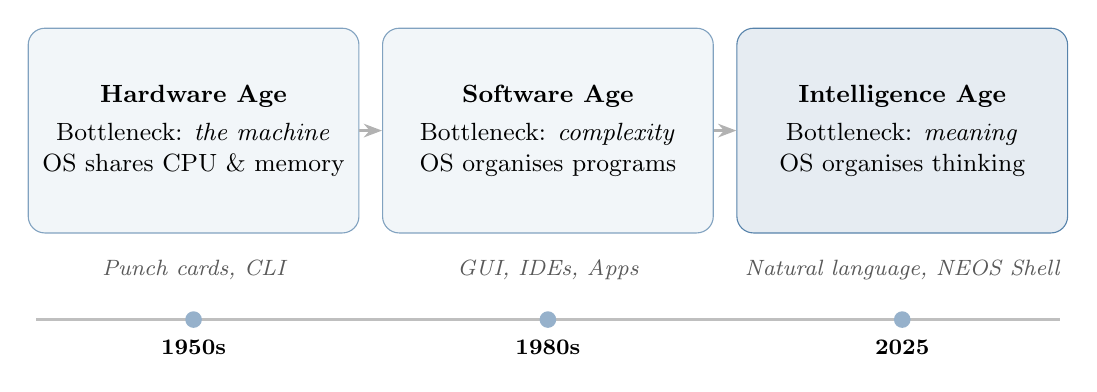
\begin{tikzpicture}[
    era/.style={
      rectangle, rounded corners=6pt, draw=neosblue!60, fill=neosblue!6,
      minimum width=4.2cm, minimum height=2.6cm, align=center,
      font=\small,
    },
    label/.style={font=\footnotesize\itshape, text=gray!70!black},
    >=Stealth
  ]

  %% --- timeline ---
  \draw[gray!50, very thick] (-6.5,0) -- (6.5,0);
  \foreach \x/\yr in {-4.5/1950s, 0/1980s, 4.5/2025} {
    \fill[neosblue!50] (\x,0) circle (3pt);
    \node[below=4pt, font=\footnotesize\bfseries] at (\x,0) {\yr};
  }

  %% --- era boxes ---
  \node[era] (hw) at (-4.5,2.4)
    {\textbf{Hardware Age}\\[3pt]
     Bottleneck: \emph{the machine}\\
     OS shares CPU \& memory};

  \node[era] (sw) at (0,2.4)
    {\textbf{Software Age}\\[3pt]
     Bottleneck: \emph{complexity}\\
     OS organises programs};

  \node[era, draw=neosblue!80, fill=neosblue!12] (ia) at (4.5,2.4)
    {\textbf{Intelligence Age}\\[3pt]
     Bottleneck: \emph{meaning}\\
     OS organises thinking};

  %% --- interface labels ---
  \node[label, below=6pt] at (hw.south) {Punch cards, CLI};
  \node[label, below=6pt] at (sw.south) {GUI, IDEs, Apps};
  \node[label, below=6pt] at (ia.south) {Natural language, NEOS Shell};

  %% --- arrows ---
  \draw[->, thick, gray!60] (hw.east) -- (sw.west);
  \draw[->, thick, gray!60] (sw.east) -- (ia.west);
\end{tikzpicture}
\caption{The three ages of computing.  Each era is defined by a
  dominant bottleneck and a corresponding OS paradigm.  The Intelligence
  Age shifts the bottleneck from hardware or software to meaning
  itself.}
\label{fig:three-ages}
\end{figure}

In the \textbf{Hardware Age} (1950s--1980s), the CPU was the scarcest
resource.  Operating systems were born to answer a single question:
\emph{How do we share this machine?}  Every cycle was a resource to be
scheduled; every byte was territory to be managed.  Batch processing,
time-sharing, and virtual memory were all answers to the hardware
bottleneck.

In the \textbf{Software Age} (1980s--2020s), hardware became abundant,
but complexity became the enemy.  C, Java, Python---humans learned
programming languages to organise millions of lines of code.  Operating
systems evolved to answer: \emph{How do we organise these programs?}
Graphical user interfaces, multitasking, and application ecosystems
arose to tame software complexity.

Now the bottleneck has moved again.  The challenge is no longer
computing faster or organising more code---it is organising
\textbf{thinking itself}.  How do you represent an idea so that it can
interact with other ideas?  How do you track which interpretations are
gaining strength?  How do you merge two lines of reasoning?  How do you
\emph{debug a thought}?  These are the questions that an OS for the
Intelligence Age must answer.  They are precisely the questions NEOS was
designed to address.

\begin{calloutbox}
The central thesis of this paper is that the next abstraction layer
will not manage code---it will manage \textbf{reasoning} as a
first-class computational primitive.
\end{calloutbox}

%% ────────────────────────────────────────────────────────────────────
\subsection{The Vision: LLM as Universal OS}\label{sec:vision}

Today, large language models are \emph{applications} that run on an
operating system---Windows, Linux, macOS~\cite{brown2020language}.
They are apps.  Useful apps, even transformative apps.  But still:
apps.

\textbf{Tomorrow, the LLM \emph{is} the operating system.}  Every
interaction with a computer will pass through language understanding.
This is not speculation---it is the trajectory we are already on.  And
NEOS is the first specification for what that world looks like.

\begin{figure}[htbp]
\centering
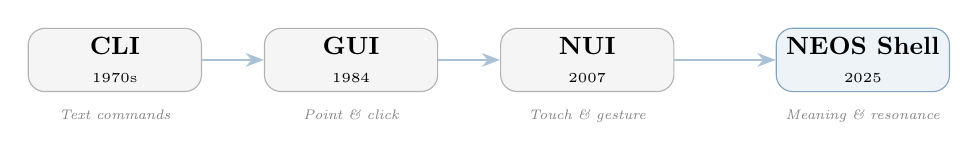
\begin{tikzpicture}[
    ibox/.style={
      rectangle, rounded corners=6pt, draw=#1!60, fill=#1!8,
      minimum width=2.2cm, minimum height=0.7cm,
      align=center, font=\small
    },
    ibox/.default=gray,
    arr/.style={-Stealth, thick, neosblue!40},
  ]
  %% --- Interface evolution ---
  \node[ibox=gray]   (cli)  at (0,0)   {\textbf{CLI}\\[-1pt]\tiny 1970s};
  \node[ibox=gray]   (gui)  at (3,0)   {\textbf{GUI}\\[-1pt]\tiny 1984};
  \node[ibox=gray]   (nui)  at (6,0)   {\textbf{NUI}\\[-1pt]\tiny 2007};
  \node[rectangle, rounded corners=6pt, draw=neosblue!60, fill=neosblue!8, minimum width=2.2cm, minimum height=0.7cm, align=center, font=\small]   (neos) at (9.5,0) {\textbf{NEOS Shell}\\[-1pt]\tiny 2025};

  \draw[arr] (cli)  -- (gui);
  \draw[arr] (gui)  -- (nui);
  \draw[arr] (nui)  -- (neos);

  \node[below=3pt, font=\tiny\itshape, text=gray] at (cli.south)
    {Text commands};
  \node[below=3pt, font=\tiny\itshape, text=gray] at (gui.south)
    {Point \& click};
  \node[below=3pt, font=\tiny\itshape, text=gray] at (nui.south)
    {Touch \& gesture};
  \node[below=3pt, font=\tiny\itshape, text=gray] at (neos.south)
    {Meaning \& resonance};
\end{tikzpicture}
\caption{Interface evolution from command-line to meaning-based
  interaction.  Each transition raises the level of abstraction at which
  humans communicate with machines.}
\label{fig:interface-evolution}
\end{figure}

Consider what this inversion means in concrete terms:

\begin{center}
\small
\begin{tabular}{@{}ll@{}}
\toprule
\thead{Old World} & \thead{New World} \\
\midrule
File systems organise by path
  & Semantic fields organise by meaning \\
Compiled binaries execute instructions
  & Field configurations execute reasoning \\
Separate applications for each task
  & Task definitions compose into workflows \\
GUIs mediate human--machine interaction
  & Natural language + shell for precision \\
\bottomrule
\end{tabular}
\end{center}

\begin{figure}[htbp]
\centering
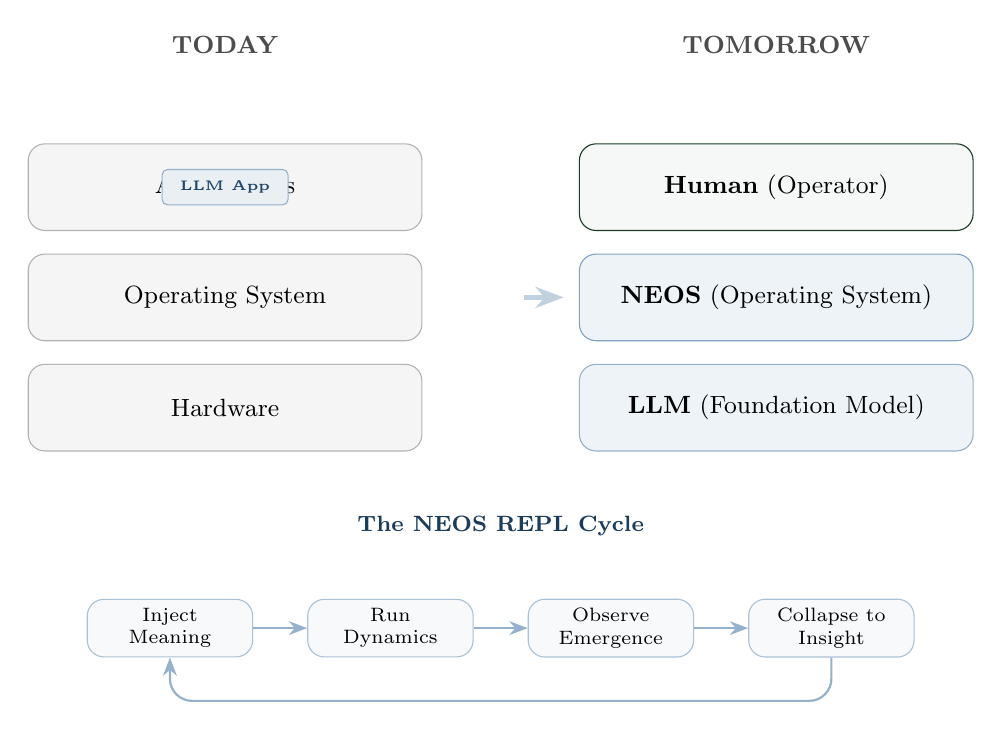
\begin{tikzpicture}[
    layer/.style={
      rectangle, rounded corners=6pt, draw=#1!60, fill=#1!8,
      minimum width=5cm, minimum height=1.1cm,
      align=center, font=\small
    },
    layer/.default=gray,
    lbl/.style={font=\small\bfseries, text=gray!60!black},
    >=Stealth
  ]

  %% ===== TODAY stack (left) =====
  \node[lbl] at (-3.5,4.6) {TODAY};

  \node[layer=gray] (thw)  at (-3.5,0)   {Hardware};
  \node[layer=gray] (tos)  at (-3.5,1.4) {Operating System};
  \node[layer=gray] (tapp) at (-3.5,2.8) {Applications};

  %% Small LLM box inside Applications
  \node[rectangle, rounded corners=2pt, draw=neosblue!50, fill=neosblue!10,
        minimum width=1.6cm, minimum height=0.45cm,
        font=\tiny\bfseries, text=neosblue!70!black]
    (llmbox) at (-3.5,2.8) {LLM App};

  %% ===== TOMORROW stack (right) =====
  \node[lbl] at (3.5,4.6) {TOMORROW};

  \node[rectangle, rounded corners=6pt, draw=neosblue!50, fill=neosblue!8,
        minimum width=5cm, minimum height=1.1cm, align=center, font=\small]
    (nfound) at (3.5,0) {\textbf{LLM} (Foundation Model)};
  \node[rectangle, rounded corners=6pt, draw=neosblue!60, fill=neosblue!8,
        minimum width=5cm, minimum height=1.1cm, align=center, font=\small] (nneos) at (3.5,1.4)
    {\textbf{NEOS} (Operating System)};
  \node[rectangle, rounded corners=6pt, draw=neosgreen!50!black, fill=neosgreen!5,
        minimum width=5cm, minimum height=1.1cm, align=center, font=\small]
    (nhum) at (3.5,2.8) {\textbf{Human} (Operator)};

  %% --- Arrow between stacks ---
  \draw[->, ultra thick, neosblue!30] (0.3,1.4) -- (0.8,1.4);

  %% ===== REPL Cycle below =====
  \node[font=\footnotesize\bfseries, text=neosblue!60!black]
    at (0, -1.5) {The NEOS REPL Cycle};

  \node[rectangle, rounded corners=6pt, draw=neosblue!40, fill=neosblue!4,
        minimum width=2.1cm, minimum height=0.65cm,
        font=\scriptsize, align=center] (r1) at (-4.2,-2.8) {Inject\\Meaning};
  \node[rectangle, rounded corners=6pt, draw=neosblue!40, fill=neosblue!4,
        minimum width=2.1cm, minimum height=0.65cm,
        font=\scriptsize, align=center] (r2) at (-1.4,-2.8) {Run\\Dynamics};
  \node[rectangle, rounded corners=6pt, draw=neosblue!40, fill=neosblue!4,
        minimum width=2.1cm, minimum height=0.65cm,
        font=\scriptsize, align=center] (r3) at (1.4,-2.8) {Observe\\Emergence};
  \node[rectangle, rounded corners=6pt, draw=neosblue!40, fill=neosblue!4,
        minimum width=2.1cm, minimum height=0.65cm,
        font=\scriptsize, align=center] (r4) at (4.2,-2.8) {Collapse to\\Insight};

  \draw[->, thick, neosblue!50] (r1) -- (r2);
  \draw[->, thick, neosblue!50] (r2) -- (r3);
  \draw[->, thick, neosblue!50] (r3) -- (r4);
  \draw[->, thick, neosblue!50, rounded corners=8pt]
    (r4.south) -- ++(0,-0.55) -| (r1.south);
\end{tikzpicture}
\caption{The architecture inversion.  \textbf{Left:} today's stack,
  where the LLM is an application running on a traditional OS.
  \textbf{Right:} the NEOS stack, where the LLM \emph{is} the
  substrate and NEOS provides the operating-system layer.
  \textbf{Bottom:} the NEOS REPL cycle---inject meaning, run dynamics,
  observe emergence, collapse to insight---with a feedback loop through
  save, fork, and share.}
\label{fig:architecture-inversion}
\end{figure}

The NEOS shell---\texttt{nf}---is the \textbf{REPL of cognitive
computing}.  The operator does not write code; instead, they inject
meaning, run dynamics, observe emergence, and collapse to insight
(Figure~\ref{fig:architecture-inversion}).  Chain-of-thought
reasoning~\cite{wei2022chain} demonstrated that LLMs can decompose
complex problems step by step; NEOS generalises this insight into a
full dynamical framework where reasoning steps are not linear chains
but interacting fields that self-organise through resonance.

``Programs'' in NEOS are not instruction sequences.  They are
\textbf{field configurations}---patterns with activation strengths,
resonance relationships, and tuneable parameters.  A program is a
thought, formalised.


\section{Architecture and Foundations}\label{sec:architecture}

NEOS v1.0 is a \textbf{specification}---37 markdown files that define
an interactive runtime environment running \emph{on} an LLM.  The LLM
is the virtual machine.  NEOS is the operating system.  Neural fields
are the computational substrate.

This section presents the governing dynamics and the three
foundational pillars on which the entire system rests.

%% ════════════════════════════════════════════════════════════════════
\subsection{The Master Equation}\label{sec:master-equation}

All dynamics in NEOS are governed by a single partial differential
equation:

\begin{eqbox}
\begin{equation}\label{eq:master-pde}
\frac{\partial A}{\partial t}
  = \underbrace{-\lambda\, A(x)}_{\text{Decay}}
  + \underbrace{\alpha \int K(x,y)\, A(y)\, dy}_{\text{Resonance}}
  + \underbrace{\iota(x,t)}_{\text{Injection}}
\end{equation}
\end{eqbox}

\noindent
This equation belongs to the family of neural field
equations introduced by Amari~\cite{amari1977dynamics} and
Wilson--Cowan~\cite{wilson1972excitatory}, adapted here for a semantic
rather than neural substrate.  Each term plays a distinct cognitive
role:

\begin{description}[leftmargin=2.2cm, labelwidth=2cm, style=nextline]

\item[\boldmath$-\lambda\, A(x)$\unboldmath\quad Decay.]
  Unreinforced ideas fade exponentially.  This is not a defect but a
  design principle: \emph{forgetting is a feature, not a bug}.  In the
  absence of resonance support, every pattern loses activation at rate
  $\lambda$, ensuring that the field does not accumulate noise
  indefinitely.  After the decay phase of each cycle, the activation
  update is $A \leftarrow A \times (1 - \lambda)$.

\item[\boldmath$\alpha \int K(x,y)\, A(y)\, dy$\unboldmath\quad Resonance.]
  Related ideas strengthen each other.  The resonance kernel
  $K(x,y)$ quantifies the semantic, logical, and contextual affinity
  between patterns located at positions $x$ and $y$ in the field.
  When two patterns resonate, each contributes to the other's
  activation proportionally to their affinity and their current
  strength.  The amplification factor $\alpha$ controls how aggressively
  mutual reinforcement operates.  This integral is the ``hearing''
  mechanism: a pattern survives not because it is loud, but because it
  is \emph{heard} by others.

\item[\boldmath$\iota(x,t)$\unboldmath\quad Injection.]
  The user adds new ideas at any time via the \texttt{nf inject}
  command.  Each injection introduces a fresh signal---a pattern with
  an initial activation strength---into the field at position $x$ and
  time $t$.  The injected pattern immediately begins interacting with
  all existing patterns through the resonance integral.

\end{description}

\noindent
From this single equation, \emph{all} of NEOS emerges: attractor
formation, coherence dynamics, collapse, versioning, and multi-field
orchestration.

\paragraph{Parameters.}
Four scalar parameters define the \textbf{cognitive style} of a field.
A security analysis benefits from low $\lambda$ (do not forget
threats), high $\alpha$ (cluster related threats fast), and high $\tau$
(only credible concerns survive).  A creative brainstorm benefits from
high $\lambda$ (rapid turnover), moderate $\alpha$, and low $\tau$
(let weak ideas live).  Same engine; different cognitive personality;
tuned with four numbers.

\begin{table}[htbp]
\centering
\caption{Master-equation parameters and their effects on field
  dynamics.}
\label{tab:parameters}
\small
\begin{tabular}{@{}cllcl@{}}
\toprule
\thead{Symbol} & \thead{Name} & \thead{Default}
  & \thead{Range} & \thead{Effect} \\
\midrule
$\lambda$ & Decay rate     & 0.05 & $[0,\,1]$
  & Higher $=$ faster forgetting \\
$\alpha$  & Amplification  & 0.30 & $[0,\,1]$
  & Higher $=$ stronger resonance \\
$\tau$    & Threshold      & 0.40 & $[0,\,1]$
  & Below this, patterns marked dormant \\
$\sigma$  & Bandwidth      & 0.50 & $[0,\,\infty)$
  & Semantic reach of each pattern \\
\bottomrule
\end{tabular}
\end{table}

%% ════════════════════════════════════════════════════════════════════
\subsection{Neural Fields --- The Substrate}\label{sec:pillar-fields}

Classical prompt engineering represents information as a linear
sequence of tokens with a hard context-window boundary.  NEOS replaces
this with \textbf{continuous activation landscapes}---neural fields in
which information is encoded not as discrete tokens but as spatially
extended activation patterns~\cite{amari1977dynamics}.

Five principles govern the substrate:

\begin{enumerate}[label=\textbf{\arabic*.}, leftmargin=2em]
\item \textbf{Continuity.}  Activation is a continuous function over a
  semantic space, not a discrete list.  Nearby meanings have nearby
  activations.

\item \textbf{Resonance.}  Patterns influence one another through the
  kernel $K(x,y)$.  If two ideas are semantically proximate, injecting
  one raises the activation of the other.

\item \textbf{Persistence.}  Information persists through resonance
  support, not through explicit inclusion in a prompt.  A pattern
  endures as long as the field sustains it.

\item \textbf{Entropy.}  The field tracks its own information-theoretic
  entropy, $H = -\sum p_i \log_2 p_i$, providing a scalar measure of
  how concentrated or diffuse the current state is.

\item \textbf{Boundary Dynamics.}  Patterns near the activation
  threshold $\tau$ are in a critical zone: small resonance boosts can
  save them, small decays can extinguish them.  This boundary behaviour
  produces the field's sensitivity to context.
\end{enumerate}

\paragraph{Why fields beat prompts.}
In a prompt, information persists only if explicitly included.  Context
window overflow silently destroys old information.  In a neural field,
information persists through \emph{resonance}---if a pattern connects
to others that keep it alive, it endures.  Relationships emerge
naturally from semantic proximity.  New input interacts with the
\emph{entire} field, not just recent tokens.

%% ════════════════════════════════════════════════════════════════════
\subsection{Symbolic Reasoning --- The Structure}\label{sec:pillar-symbolic}

Without structure, fields are beautiful but unusable---like having a
piano with no keys.  The \texttt{nf} command set provides the
\textbf{opcodes of cognitive computing}: a symbolic language for field
manipulation that is both human-readable and algebraically precise.

Core operations include:
\texttt{inject} (add a pattern),
\texttt{amplify} (increase activation),
\texttt{attenuate} (decrease activation),
\texttt{cycle} (advance dynamics),
\texttt{collapse} (resolve superposition), and
\texttt{commit} (snapshot state).
Each command has a precise mathematical meaning in terms of the master
equation~\eqref{eq:master-pde}.

Two reference conventions provide the symbolic glue:

\begin{itemize}[leftmargin=1.5em]
\item \textbf{Pattern references} (\texttt{@name}) select an
  individual pattern in the field.
\item \textbf{Field references} (\texttt{\$field}) select an entire
  named field in multi-field configurations.
\end{itemize}

\noindent
Operations compose algebraically.  For example, applying
\texttt{amplify(@a, 1.5)} followed by \texttt{attenuate(@a, 0.5)}
returns the pattern to a well-defined intermediate activation
that can be computed from the field state alone.

%% ════════════════════════════════════════════════════════════════════
\subsection{Quantum Semantics --- The Interpretation}%
\label{sec:pillar-quantum}

Before collapse, meaning exists in
\textbf{superposition}~\cite{busemeyer2012quantum}.  The field holds
multiple possible interpretations simultaneously, each weighted by
activation strength.  This is not a loose metaphor: the mathematical
structure of NEOS's collapse operation mirrors key features of quantum
measurement~\cite{pothos2013can}.  We adopt the term ``quantum
semantics'' from the quantum cognition literature; the formalism draws
on quantum probability theory as a model of cognitive phenomena, not on
quantum physics.

\paragraph{Non-commutativity.}
Injecting pattern $A$ and then pattern $B$ is \emph{not} the same as
injecting $B$ and then $A$.  Each injection alters the field that
receives the next one.  Formally, if $I_A$ and $I_B$ denote the
injection operators, then in general $I_A \circ I_B \neq I_B \circ
I_A$ because the resonance integral couples each new pattern to the
full existing field state.  Order of inquiry shapes the space of
possible conclusions.

\paragraph{Observer-dependent collapse.}
When the operator issues \texttt{nf collapse}, the superposition
resolves into a definite output---but the result depends on the
chosen strategy:

\begin{itemize}[leftmargin=1.5em]
\item \textbf{Attractor}: select the dominant attractor basin.
\item \textbf{Threshold}: retain all patterns above a specified
  activation.
\item \textbf{Weighted}: blend all patterns proportionally to their
  activation.
\item \textbf{Sample}: probabilistically sample from the activation
  distribution.
\end{itemize}

\noindent
The observer matters.  The strategy you choose shapes the output you
get.  The same field can collapse differently under different
strategies, just as the same quantum state yields different
measurement outcomes under different observables.

%% ════════════════════════════════════════════════════════════════════
\subsection{The Three Pillars in Concert}\label{sec:pillars-unified}

\begin{figure}[H]
\centering
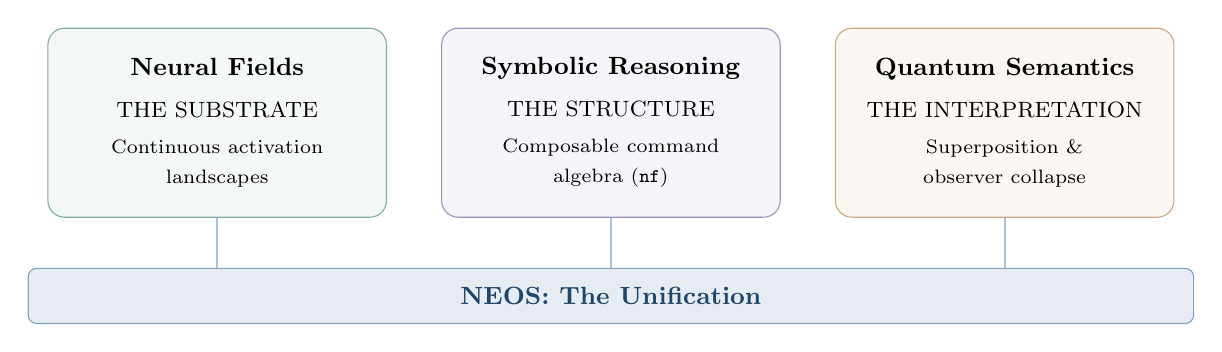
\begin{tikzpicture}[
    >=Stealth
  ]

  %% --- Three pillars ---
  \node[draw=neosteal!60, fill=neosteal!6, minimum width=4.3cm, minimum height=2.4cm, align=center, font=\small, rounded corners=6pt] (nf) at (-5,0)
    {\textbf{Neural Fields}\\[4pt]
     {\footnotesize THE SUBSTRATE}\\[2pt]
     {\scriptsize Continuous activation}\\
     {\scriptsize landscapes}};

  \node[draw=neosviolet!60, fill=neosviolet!6, minimum width=4.3cm, minimum height=2.4cm, align=center, font=\small, rounded corners=6pt] (sr) at (0,0)
    {\textbf{Symbolic Reasoning}\\[4pt]
     {\footnotesize THE STRUCTURE}\\[2pt]
     {\scriptsize Composable command}\\
     {\scriptsize algebra (\texttt{nf})}};

  \node[draw=neosorange!60, fill=neosorange!6, minimum width=4.3cm, minimum height=2.4cm, align=center, font=\small, rounded corners=6pt] (qs) at (5,0)
    {\textbf{Quantum Semantics}\\[4pt]
     {\footnotesize THE INTERPRETATION}\\[2pt]
     {\scriptsize Superposition \&}\\
     {\scriptsize observer collapse}};

  %% --- Unification bar ---
  \node[rectangle, rounded corners=3pt, draw=neosblue!60, fill=neosblue!12,
        minimum width=14.8cm, minimum height=0.7cm,
        font=\small\bfseries, text=neosblue!70!black]
    (bar) at (0,-2.2) {NEOS: The Unification};

  %% --- Connections ---
  \draw[thick, neosblue!40] (nf.south)  -- (bar.north -| nf.south);
  \draw[thick, neosblue!40] (sr.south)  -- (bar.north);
  \draw[thick, neosblue!40] (qs.south)  -- (bar.north -| qs.south);
\end{tikzpicture}
\caption{The three pillars of NEOS.  Neural fields provide the
  computational substrate; symbolic reasoning provides the structural
  language; quantum semantics provides the interpretive framework.
  NEOS unifies all three into a single coherent system.}
\label{fig:three-pillars}
\end{figure}

Each pillar is necessary; together they make cognitive computing
possible.  Remove neural fields and the system cannot \emph{represent}
meaning.  Remove symbolic reasoning and it cannot \emph{manipulate}
meaning.  Remove quantum semantics and it cannot \emph{interpret}
meaning.  Figure~\ref{fig:three-pillars} shows the relationship.

\paragraph{Collapse visualised.}
Figure~\ref{fig:quantum-collapse} illustrates the collapse operation.
Before collapse, the field contains multiple patterns in superposition,
each with a distinct activation level.  After the operator issues
\texttt{nf collapse}, the superposition resolves into structured
output---the dominant interpretation crystallised from the full field
state.

\begin{figure}[H]
\centering
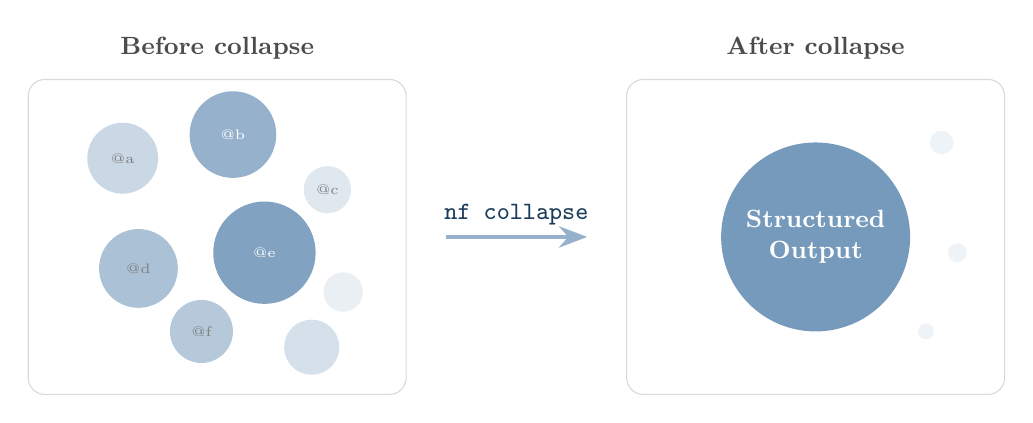
\begin{tikzpicture}[>=Stealth]

  %% ===== BEFORE (left panel) =====
  \node[font=\small\bfseries, text=gray!60!black] at (-3.8,2.6)
    {Before collapse};

  \draw[gray!30, rounded corners=6pt]
    (-6.2,-1.8) rectangle (-1.4,2.2);

  % Multiple patterns (circles of varying size/shade)
  \fill[neosblue!25]   (-5.0, 1.2) circle (0.45);
  \fill[neosblue!50]   (-3.6, 1.5) circle (0.55);
  \fill[neosblue!15]   (-2.4, 0.8) circle (0.30);
  \fill[neosblue!40]   (-4.8,-0.2) circle (0.50);
  \fill[neosblue!60]   (-3.2, 0.0) circle (0.65);
  \fill[neosblue!10]   (-2.2,-0.5) circle (0.25);
  \fill[neosblue!35]   (-4.0,-1.0) circle (0.40);
  \fill[neosblue!20]   (-2.6,-1.2) circle (0.35);

  % Labels
  \node[font=\tiny, text=gray] at (-5.0, 1.2) {@a};
  \node[font=\tiny, text=white] at (-3.6, 1.5) {@b};
  \node[font=\tiny, text=gray] at (-2.4, 0.8) {@c};
  \node[font=\tiny, text=gray] at (-4.8,-0.2) {@d};
  \node[font=\tiny, text=white] at (-3.2, 0.0) {@e};
  \node[font=\tiny, text=gray] at (-4.0,-1.0) {@f};

  %% ===== ARROW =====
  \draw[->, ultra thick, neosblue!50] (-0.9,0.2) -- (0.9,0.2)
    node[midway, above, font=\small\bfseries, text=neosblue!60!black]
      {\texttt{nf collapse}};

  %% ===== AFTER (right panel) =====
  \node[font=\small\bfseries, text=gray!60!black] at (3.8,2.6)
    {After collapse};

  \draw[gray!30, rounded corners=6pt]
    (1.4,-1.8) rectangle (6.2,2.2);

  % Single dominant circle
  \fill[neosblue!65] (3.8,0.2) circle (1.2);
  \node[font=\small\bfseries, text=white, align=center] at (3.8,0.2)
    {Structured\\Output};

  % Faint remnants
  \fill[neosblue!8] (5.4, 1.4) circle (0.15);
  \fill[neosblue!8] (5.6, 0.0) circle (0.12);
  \fill[neosblue!8] (5.2,-1.0) circle (0.10);

\end{tikzpicture}
\caption{Field collapse (quantum-inspired semantics).  \textbf{Left:} the field in
  superposition---multiple patterns with varying activation levels.
  \textbf{Right:} after \texttt{nf collapse}, the dominant
  interpretation crystallises into structured output.  Residual
  patterns fade to near-zero activation.}
\label{fig:quantum-collapse}
\end{figure}


% ══════════════════════════════════════════════════════════════════
%  Section 3 — The JVM Analogy
% ══════════════════════════════════════════════════════════════════

\section{The JVM Analogy}\label{sec:analogy}

In 1995, Java promised \emph{``Write once, run anywhere.''}  The Java
Virtual Machine decoupled application code from the underlying hardware:
a developer could compile once and deploy on any platform that hosted
a conforming JVM.  The insight was that \textbf{execution} need not be
bound to a specific processor architecture.

NEOS makes an analogous promise one abstraction level higher:
\emph{``Think once, reason anywhere.''}  NEOS decouples
\textbf{reasoning} from any specific large language model.  Whether the
substrate is GPT-4, Claude, Gemini, Llama, or a model that does not yet
exist, the field dynamics, attractor basins, and collapse operators
behave identically---just as a Java program behaves identically on x86
and ARM.

The parallel is not merely rhetorical.  Table~\ref{tab:jvm-neos}
enumerates six structural correspondences between the JVM runtime and
the NEOS runtime, each grounded in a shared engineering insight.

% ── JVM vs NEOS table ────────────────────────────────────────────
\begin{table}[htbp]
\centering
\caption{Structural correspondences between the JVM and NEOS runtimes.}
\label{tab:jvm-neos}
\begin{tabularx}{\textwidth}{@{}llX@{}}
\toprule
\thead{JVM World} & \thead{NEOS World} & \thead{The Insight} \\
\midrule
Garbage Collection  & Decay ($\lambda$)
  & Automatic cleanup of unreferenced objects\,/\,unreinforced patterns \\
Heap Memory         & Field State
  & Where objects\,/\,patterns live and interact \\
Threads             & Multi-Field
  & Concurrent execution contexts with shared state \\
Stack Trace         & Cycle Trace
  & Debugging by tracing execution\,/\,dynamics history \\
ClassLoader         & Pattern Injection
  & Loading new code\,/\,meaning into the runtime \\
JIT Compilation     & Adaptive Resonance
  & Runtime optimisation based on actual usage patterns \\
\bottomrule
\end{tabularx}
\end{table}

\paragraph{The key argument.}
The JVM abstracted \emph{hardware}; NEOS abstracts \emph{cognition
itself}.  The JVM executes \textbf{code}---deterministic instruction
sequences that transform data.  NEOS executes \textbf{meaning}---patterns
that interact through resonance, compete for activation energy, and
self-organise into attractor basins.  Code is brittle: change one
instruction and the program crashes.  Meaning is robust: perturb a
pattern and the field relaxes back toward its attractors, provided the
perturbation falls within the basin of attraction.

\paragraph{The garbage-collection parallel.}
The correspondence between garbage collection and decay~($\lambda$)
deserves special attention.  In the JVM, the garbage collector reclaims
heap memory occupied by objects that are no longer reachable from any
live reference.  In NEOS, the decay term
$-\lambda\,A(x)$ continuously diminishes the activation of every pattern
that is not sustained by resonance with its neighbours.  Both mechanisms
solve the same fundamental problem---\emph{resource accumulation}---at
different abstraction levels: the JVM prevents memory leaks, NEOS
prevents \emph{semantic leaks}, the unbounded growth of irrelevant ideas
that would otherwise drown out meaningful signal.

% ── TikZ: JVM vs NEOS parallel stacks ───────────────────────────
\begin{figure}[htbp]
\centering
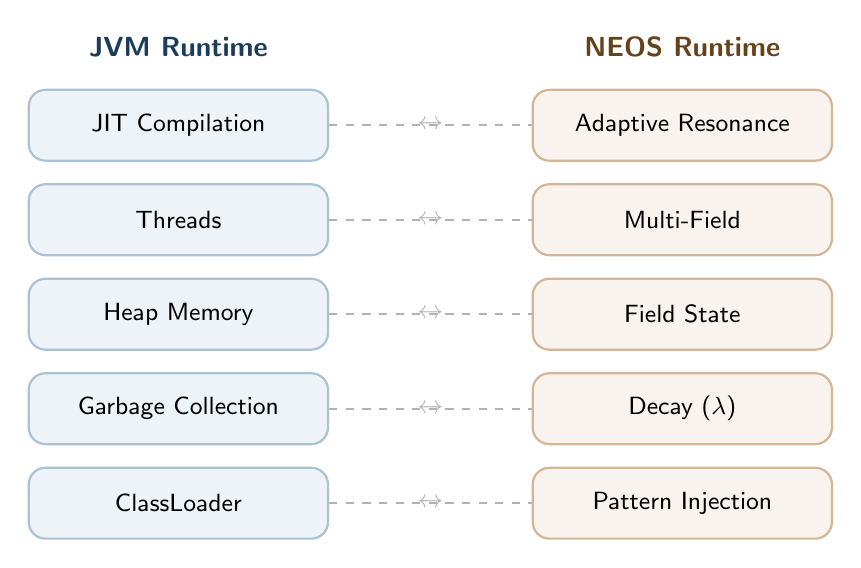
\begin{tikzpicture}[
  box/.style={
    draw, rounded corners=6pt, minimum width=3.8cm, minimum height=0.9cm,
    font=\small\sffamily, align=center, thick,
  },
  jvmbox/.style={box, fill=neosblue!8, draw=neosblue!40},
  neosbox/.style={box, fill=neosorange!8, draw=neosorange!50},
  conn/.style={dashed, gray!60, thick},
  lbl/.style={font=\footnotesize\sffamily, gray!70},
]

% Column titles
\node[font=\bfseries\sffamily, neosblue!60!black] at (-3.2, 5.8) {JVM Runtime};
\node[font=\bfseries\sffamily, neosorange!60!black] at ( 3.2, 5.8) {NEOS Runtime};

% Left column — JVM (top to bottom)
\node[jvmbox] (jit)  at (-3.2, 4.8) {JIT Compilation};
\node[jvmbox] (thr)  at (-3.2, 3.6) {Threads};
\node[jvmbox] (heap) at (-3.2, 2.4) {Heap Memory};
\node[jvmbox] (gc)   at (-3.2, 1.2) {Garbage Collection};
\node[jvmbox] (cl)   at (-3.2, 0.0) {ClassLoader};

% Right column — NEOS (top to bottom)
\node[neosbox] (ar)   at (3.2, 4.8) {Adaptive Resonance};
\node[neosbox] (mf)   at (3.2, 3.6) {Multi-Field};
\node[neosbox] (fs)   at (3.2, 2.4) {Field State};
\node[neosbox] (dec)  at (3.2, 1.2) {Decay ($\lambda$)};
\node[neosbox] (pi)   at (3.2, 0.0) {Pattern Injection};

% Dashed connections with centered arrows
\foreach \l/\r in {jit/ar, thr/mf, heap/fs, gc/dec, cl/pi} {
  \draw[conn] (\l.east) -- (\r.west)
    node[midway, font=\small] {$\leftrightarrow$};
}

\end{tikzpicture}
\caption{Parallel runtime stacks.  Each layer of the JVM has a
  structural correspondent in NEOS, operating on meaning rather than
  data.}
\label{fig:jvm-neos-stacks}
\end{figure}

Just as the JVM freed developers from thinking about registers and
calling conventions, NEOS frees analysts from thinking about prompt
engineering and model-specific idiosyncrasies.  The abstraction
boundary is the field equation: everything above it speaks the
language of patterns and resonance; everything below it is an
implementation detail of the substrate.


% ══════════════════════════════════════════════════════════════════
%  Section 4 — System Design
% ══════════════════════════════════════════════════════════════════

\section{System Design}\label{sec:system}

This section describes the four principal subsystems of NEOS---the
command interface, the field dynamics engine, the multi-field
orchestrator, and the interface layer---followed by a walkthrough of the
interactive shell.

% ─────────────────────────────────────────────────────────────────
\subsection{Command Interface}\label{sec:command-interface}

Every interaction with NEOS follows a single syntactic template:

\medskip
\begin{center}
\texttt{nf <command> [subcommand] [arguments] [-{}-flags]}
\end{center}
\medskip

\noindent
Patterns are referenced with the \texttt{@name} sigil; fields with
\texttt{\$field}.  The design is deliberately Unix-flavoured:
\emph{imperative verbs acting on semantic objects}.  Commands are
organised into six categories:

\begin{enumerate}[nosep]
  \item \textbf{Operations} --- create, inject, remove, and transform
        patterns.
  \item \textbf{Dynamics} --- advance the field through cycles, control
        decay and resonance parameters.
  \item \textbf{Measurement} --- query activation, coherence, energy,
        and attractor membership.
  \item \textbf{Visualisation} --- render field state as landscapes,
        graphs, and heatmaps.
  \item \textbf{Versioning} --- commit, branch, and diff field states.
  \item \textbf{Autonomy} --- define tasks that run to a convergence
        criterion without user intervention.
\end{enumerate}

% ── TikZ: Command pipeline ──────────────────────────────────────
\begin{figure}[htbp]
\centering
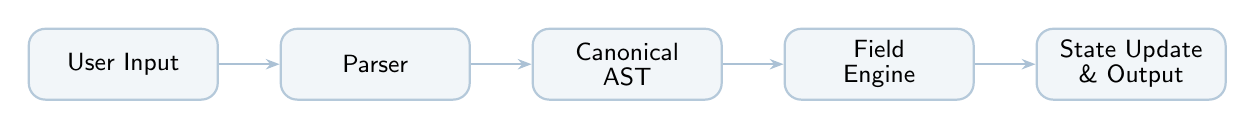
\begin{tikzpicture}[
  stage/.style={
    draw, rounded corners=6pt, fill=neosblue!6, draw=neosblue!35,
    minimum width=2.4cm, minimum height=0.9cm,
    font=\small\sffamily, align=center, thick
  },
  arr/.style={-{Stealth[length=5pt]}, thick, neosblue!40},
]

\node[stage] (inp)    at (0,0)    {User Input};
\node[stage] (parse)  at (3.2,0)  {Parser};
\node[stage] (ast)    at (6.4,0)  {Canonical\\[-2pt]AST};
\node[stage] (eng)    at (9.6,0)  {Field\\[-2pt]Engine};
\node[stage] (out)    at (12.8,0) {State Update\\[-2pt]\& Output};

\draw[arr] (inp)   -- (parse);
\draw[arr] (parse) -- (ast);
\draw[arr] (ast)   -- (eng);
\draw[arr] (eng)   -- (out);

\end{tikzpicture}
\caption{Command pipeline.  Every interaction, regardless of input
  modality, is parsed into the same Canonical AST before reaching the
  field engine.}
\label{fig:command-pipeline}
\end{figure}

% ─────────────────────────────────────────────────────────────────
\subsection{Field Dynamics}\label{sec:field-dynamics}

Each invocation of \texttt{nf cycle} advances the field through six
sequential phases:

\begin{enumerate}[nosep]
  \item \textbf{Decay.}\quad $A \leftarrow A \times (1 - \lambda)$.
        Every pattern loses a fixed fraction of its activation, ensuring
        that unreinforced ideas fade.
  \item \textbf{Resonate.}\quad Pairwise resonance is computed across
        semantic, logical, and contextual dimensions.
  \item \textbf{Amplify.}\quad
        $A \leftarrow A + \alpha \sum (R \cdot A)$.
        Patterns that resonate strongly with their neighbours gain
        activation energy.
  \item \textbf{Threshold.}\quad $A < \tau \;\Rightarrow\;
        \text{mark dormant}$.  Patterns whose activation has fallen
        below a critical value are flagged as dormant and excluded from
        further resonance computation.
  \item \textbf{Coherence.}\quad
        $C = \mu_R\, / \,(1 + \sigma^{2}_R)$.
        A scalar summary of how tightly the surviving patterns agree.
  \item \textbf{Attractor.}\quad Emergence is declared when three
        conditions hold simultaneously:
        coherence $> 0.6$, energy $> 70\%$ of maximum, and
        perturbation-stability under small noise.
\end{enumerate}

% ── TikZ: Six-phase dynamics ring ────────────────────────────────
\begin{figure}[htbp]
\centering
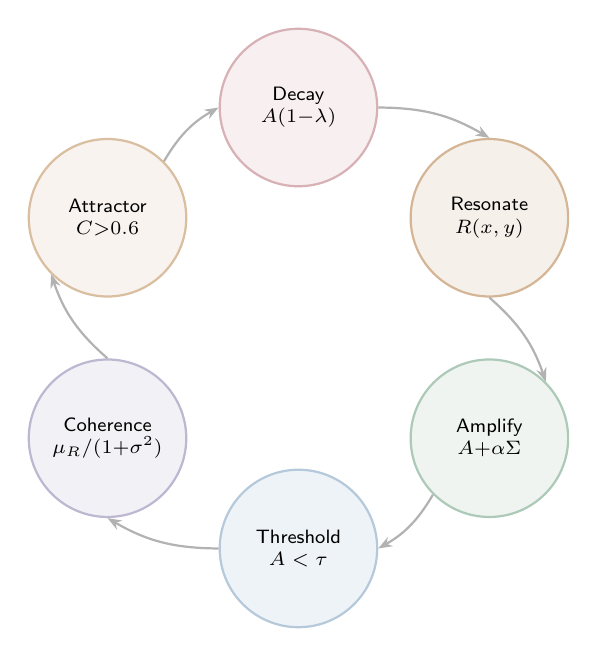
\begin{tikzpicture}[
  phase/.style={
    draw, circle, minimum size=2.0cm, thick,
    font=\scriptsize\sffamily, align=center, inner sep=2pt
  },
  arr/.style={-{Stealth[length=5pt]}, thick, gray!60},
]

% Place six nodes in a hexagonal ring (starting from top, clockwise)
\def\R{2.8}
\node[phase, fill=neosred!8,    draw=neosred!40]
  (p1) at (90:\R)  {Decay\\$A(1{-}\lambda)$};
\node[phase, fill=neosorange!10, draw=neosorange!50]
  (p2) at (30:\R)  {Resonate\\$R(x,y)$};
\node[phase, fill=neosgreen!8,  draw=neosgreen!40]
  (p3) at (-30:\R) {Amplify\\$A{+}\alpha\Sigma$};
\node[phase, fill=neosblue!8,   draw=neosblue!35]
  (p4) at (-90:\R) {Threshold\\$A<\tau$};
\node[phase, fill=neosviolet!8, draw=neosviolet!40]
  (p5) at (210:\R) {Coherence\\$\mu_R/(1{+}\sigma^2)$};
\node[phase, fill=neosorange!8, draw=neosorange!45]
  (p6) at (150:\R) {Attractor\\$C{>}0.6$};

% Clockwise arrows
\draw[arr] (p1.east)  to[bend left=15] (p2.north);
\draw[arr] (p2.south) to[bend left=15] (p3.north east);
\draw[arr] (p3.south west) to[bend left=15] (p4.east);
\draw[arr] (p4.west)  to[bend left=15] (p5.south);
\draw[arr] (p5.north) to[bend left=15] (p6.south west);
\draw[arr] (p6.north east) to[bend left=15] (p1.west);

\end{tikzpicture}
\caption{The six-phase dynamics ring executed during each
  \texttt{nf cycle} invocation.  Arrows indicate the fixed evaluation
  order.}
\label{fig:dynamics-ring}
\end{figure}

% ─────────────────────────────────────────────────────────────────
\subsection{Multi-Field Orchestration}\label{sec:multi-field}

A single field captures one perspective.  Real problems demand several.
NEOS supports multiple coupled fields---for instance, a
\emph{Technical} field, a \emph{Business} field, and a \emph{User}
field---each evolving under its own dynamics but linked through a
coupling matrix~$\Gamma$.

Stability requires that the spectral radius of~$\Gamma$ remain bounded:
\begin{equation}\label{eq:coupling-stability}
  \rho(\Gamma) \;<\; \frac{\lambda_{\min}}{\alpha_{\max}}\,,
\end{equation}
where $\lambda_{\min}$ is the smallest decay rate across fields and
$\alpha_{\max}$ is the largest amplification factor.  When
\eqref{eq:coupling-stability} is satisfied, cross-field influence is
strong enough to exchange information yet too weak to destabilise any
individual field.

Two orchestration modes are provided:

\begin{itemize}[nosep]
  \item \textbf{Pipeline} --- fields execute sequentially, each seeding
        the next with its collapsed output.
  \item \textbf{Parallel} --- fields execute simultaneously, exchanging
        activation through~$\Gamma$ at every cycle.
\end{itemize}

% ── TikZ: Multi-field orchestration ──────────────────────────────
\begin{figure}[htbp]
\centering
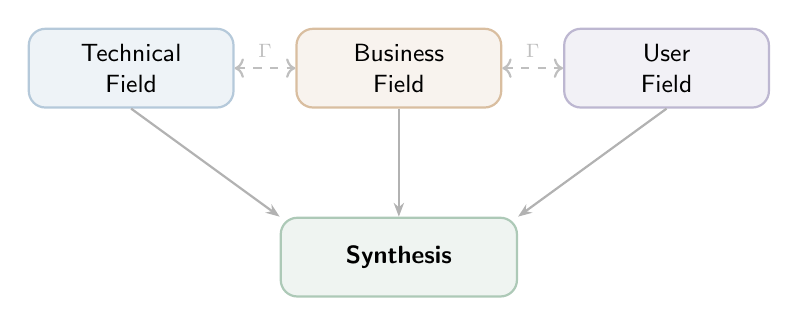
\begin{tikzpicture}[
  field/.style={
    draw, rounded corners=6pt, minimum width=2.6cm,
    minimum height=1.0cm, thick, font=\small\sffamily,
    align=center
  },
  synth/.style={
    draw, rounded corners=6pt, minimum width=3.0cm,
    minimum height=1.0cm, thick, font=\small\sffamily\bfseries,
    fill=neosgreen!8, draw=neosgreen!40, align=center
  },
  arr/.style={-{Stealth[length=5pt]}, thick, gray!60},
]

\node[field, fill=neosblue!8,   draw=neosblue!35]   (tech) at (-3.4, 2) {Technical\\Field};
\node[field, fill=neosorange!8, draw=neosorange!45]  (biz)  at ( 0.0, 2) {Business\\Field};
\node[field, fill=neosviolet!8, draw=neosviolet!40]  (usr)  at ( 3.4, 2) {User\\Field};

\node[synth] (syn) at (0, -0.4) {Synthesis};

\draw[arr] (tech.south) -- (syn.north west);
\draw[arr] (biz.south)  -- (syn.north);
\draw[arr] (usr.south)  -- (syn.north east);

% Coupling arcs between fields
\draw[dashed, gray!50, thick, <->]
  (tech.east) -- (biz.west)
  node[midway, above, font=\scriptsize\sffamily] {$\Gamma$};
\draw[dashed, gray!50, thick, <->]
  (biz.east) -- (usr.west)
  node[midway, above, font=\scriptsize\sffamily] {$\Gamma$};

\end{tikzpicture}
\caption{Multi-field orchestration.  Three perspective fields are
  coupled through~$\Gamma$ and converge into a single synthesis node.}
\label{fig:multi-field}
\end{figure}

% ─────────────────────────────────────────────────────────────────
\subsection{Interface Modes}\label{sec:interfaces}

NEOS exposes three input modalities, all of which compile to the same
Canonical AST:

\begin{enumerate}[nosep]
  \item \textbf{Semantic interface} --- natural-language statements
        parsed into field operations
        (e.g., \emph{``inject security with strength 0.9''}).
  \item \textbf{Algebraic interface} --- formal mathematical notation:
        $\iota(\text{``security''},\, 0.9)$.
  \item \textbf{Shell interface} --- the command line:
        \texttt{nf inject "security" 0.9}.
\end{enumerate}

\noindent
The three modalities are isomorphic: every expression in one can be
mechanically translated to the other two.  This triple interface ensures
that NEOS is equally accessible to domain experts (semantic), theorists
(algebraic), and engineers (shell).

% ─────────────────────────────────────────────────────────────────
\subsection{The NEOS Shell}\label{sec:shell}

The NEOS shell is a read-eval-print loop (REPL) for cognitive
computing---what \texttt{bash} is to Unix, the NEOS shell is to the
neural field.  A typical session proceeds through three phases:

\begin{description}[nosep, leftmargin=2em, labelwidth=1.8em, style=nextline]
  \item[\textnormal{\textsc{Create}}]
    Inject patterns into the field
    (\texttt{nf inject}).
  \item[\textnormal{\textsc{Compile}}]
    Collapse the superposition into a definite output
    (\texttt{nf collapse}).
  \item[\textnormal{\textsc{Run}}]
    Execute an autonomous task against a convergence criterion
    (\texttt{nf task}).
\end{description}

\noindent
Debugging a thought proceeds exactly as debugging a program: set
checkpoints (\texttt{nf checkpoint}), enter step mode
(\texttt{nf cycle 1 -{}-trace}), and inspect the cycle trace to
understand why a pattern gained or lost activation.

% ─────────────────────────────────────────────────────────────────
\subsection{Getting Started: A Walkthrough}\label{sec:tutorial}

Using NEOS requires no installation.  The operator copies the kernel
prompt (\texttt{prompts/nfos-kernel.md}) and pastes it as the system
prompt in any LLM interface that supports one.  The LLM becomes the
NEOS runtime.  The following walkthrough demonstrates the complete
analysis cycle using a startup-idea evaluation as the domain.

\paragraph*{Step~1: Create a Session.}

\begin{terminalbox}[Startup Analysis --- Session Creation]
\begin{lstlisting}[style=neosshell]
nf session new "Startup Idea Analysis"
[SESSION] Created: Startup Idea Analysis
  Field: main (default)
  Parameters: l=0.05  a=0.30  t=0.40  s=0.50
  Mode: step (interactive)
\end{lstlisting}
\end{terminalbox}

\noindent
A session initialises a default field with standard
parameters.  The operator can tune parameters at any time with
\texttt{nf tune}.

\paragraph*{Step~2: Inject Patterns.}

\begin{terminalbox}[Startup Analysis --- Pattern Injection]
\begin{lstlisting}[style=neosshell]
nf inject "strong_founding_team" 0.9
[INJECT] strong_founding_team (s: 0.90)

nf inject "crowded_market" 0.7
[INJECT] crowded_market (s: 0.70)
  [RESONANCE] <-> @strong_founding_team: R = 0.42 MODERATE

nf inject "novel_technology" 0.85
[INJECT] novel_technology (s: 0.85)

nf inject "unclear_revenue_model" 0.6
[INJECT] unclear_revenue_model (s: 0.60)

nf inject "early_traction_with_users" 0.8
[INJECT] early_traction_with_users (s: 0.80)
  [RESONANCE] <-> @strong_founding_team: R = 0.78 STRONG
\end{lstlisting}
\end{terminalbox}

\noindent
Each pattern is an observation with an activation strength
(0.0--1.0).  Higher strength indicates greater initial confidence.
Resonance is computed automatically at injection time.

\paragraph*{Step~3: Run Dynamics.}

\begin{terminalbox}[Startup Analysis --- Five Cycles]
\begin{lstlisting}[style=neosshell]
nf cycle 5 --trace
[CYCLE 1] C = 0.38
  @strong_founding_team: 0.90 -> 0.94  (resonance boost)
  @crowded_market:       0.70 -> 0.67  (decay, low resonance)
[CYCLE 2] C = 0.52
  Cluster forming: {team, traction, technology}
[CYCLE 3] C = 0.64
  [ATTRACTOR-EMERGED] "strong_fundamentals"
    Core: {@strong_founding_team, @early_traction,
           @novel_technology}
    Coherence: 0.64
[CYCLE 4] C = 0.71
[CYCLE 5] C = 0.76
  @unclear_revenue_model: 0.52 (weakening, low resonance)
  @crowded_market: 0.48 (near threshold)
\end{lstlisting}
\end{terminalbox}

\noindent
Each cycle applies the master equation: decay erodes unreinforced
patterns, resonance amplifies related ones.  The positive factors
(team, technology, traction) cluster into an attractor; risks
(crowded market, unclear revenue) weaken due to low mutual resonance.

\clearpage
\paragraph*{Step~4: Collapse to Insight.}

\begin{terminalbox}[Startup Analysis --- Collapse]
\begin{lstlisting}[style=neosshell]
nf collapse --strategy attractor
[COLLAPSE] Strategy: attractor
  Dominant: strong_fundamentals (C=0.76)

OUTPUT:
  The field identifies strong technical and team fundamentals
  with early market validation.  Primary risks are an unclear
  revenue model and a crowded market---both weakening under
  dynamics, suggesting they are less structurally connected to
  the core thesis than the positive signals.

  Confidence: HIGH (0.76)
\end{lstlisting}
\end{terminalbox}

\noindent
Collapse resolves the field's superposition into structured output.
The operator can also query the field in natural language
(\texttt{nf ask "What is the biggest risk?"}), save the state
(\texttt{nf commit}), branch to explore alternatives
(\texttt{nf branch create}), or switch to autonomous mode
(\texttt{nf mode auto}) for hands-free analysis.

\medskip
\noindent
This four-step cycle---inject, run dynamics, observe, collapse---is the
fundamental workflow of NEOS.  The empirical
evidence~(\S\ref{sec:evidence}) demonstrates the same cycle operating
at scale: 69~patterns over 52~cycles in software quality, and
10~patterns over 12~cycles in network forensics.


% ======================================================================
%  Section 6 --- Advanced Capabilities
% ======================================================================

\section{Advanced Capabilities}\label{sec:advanced}

The preceding sections described NEOS as it operates on a single field
with a single operator.  This section lifts that restriction and
explores the seven capabilities that move NEOS from a reasoning tool
to a reasoning \emph{platform}: evolutionary depth, unification of
its three pillars, the historical moment that makes it buildable,
multi-agent orchestration, versioned thinking, adjustable autonomy,
and observable reasoning.

%% ─────────────────────────────────────────────────────────────────────
\subsection{Evolution Hierarchy}\label{sec:evolution}

NEOS does not emerge from nowhere.  It sits atop a progression that
mirrors the deepest organisational principle in nature: each level
encapsulates and transcends the one below.

\begin{center}
\small
\begin{tabular}{@{}rll@{}}
\toprule
\thead{Level} & \thead{Unit} & \thead{Organising Principle} \\
\midrule
1 & Atoms       & Physical forces \\
2 & Molecules   & Chemical bonds \\
3 & Cells       & Biochemical signalling \\
4 & Organs      & Tissue-level coordination \\
5 & Neuro Systems & Discrete neural circuits \\
6 & Neural Fields & Continuous functional landscapes \\
\bottomrule
\end{tabular}
\end{center}

The leap from Level~5 to Level~6 recapitulates the leap from Level~3
to Level~4.  Cells are discrete processing units; organs are
continuous functional landscapes.  Individual neurons are discrete
processing units; neural fields are continuous functional landscapes.
In both cases, the transition is marked by the same qualitative
change: the system's behaviour can no longer be understood as a sum of
its parts.  Emergent dynamics---attractors, resonance, phase
transitions---become the primary explanatory vocabulary.

NEOS lives at Level~6.  It does not simulate individual neurons or
individual prompt--response pairs.  It operates on the continuous
semantic manifold that \emph{arises from} those discrete interactions,
just as a magnetic field arises from---but is not reducible to---the
individual spins of iron atoms.

%% ─────────────────────────────────────────────────────────────────────
\subsection{The Unified Field}\label{sec:unified}

Throughout this paper we have described three pillars: neural field
dynamics, symbolic reasoning, and quantum semantics.  These are not
three independent modules bolted together.  They are three perspectives
on a single underlying reality---much as wave mechanics, matrix
mechanics, and path integrals are all quantum mechanics.

\begin{figure}[H]
\centering
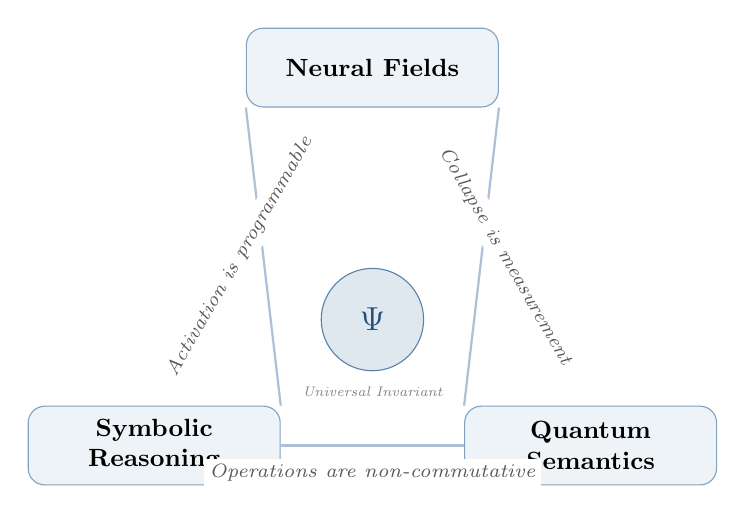
\begin{tikzpicture}[
    vtx/.style={
      rectangle, rounded corners=6pt, draw=neosblue!60, fill=neosblue!8,
      minimum width=3.2cm, minimum height=1cm,
      align=center, font=\small\bfseries
    },
    edgelbl/.style={
      font=\scriptsize\itshape, text=gray!70!black,
      fill=white, inner sep=2pt
    },
    >=Stealth
  ]

  %% Equilateral triangle vertices
  \coordinate (A) at (90:3.2);   % top
  \coordinate (B) at (210:3.2);  % bottom-left
  \coordinate (C) at (330:3.2);  % bottom-right

  %% Vertex boxes
  \node[vtx] (nf) at (A)  {Neural Fields};
  \node[vtx] (sr) at (B)  {Symbolic\\Reasoning};
  \node[vtx] (qs) at (C)  {Quantum\\Semantics};

  %% Edges
  \draw[thick, neosblue!40] (nf.south west) -- (sr.north east);
  \draw[thick, neosblue!40] (sr.east) -- (qs.west);
  \draw[thick, neosblue!40] (qs.north west) -- (nf.south east);

  %% Edge labels
  \node[edgelbl, rotate=60]  at ($(A)!0.5!(B) + (-0.3,0)$)
    {Activation is programmable};
  \node[edgelbl]             at ($(B)!0.5!(C) + (0,-0.35)$)
    {Operations are non-commutative};
  \node[edgelbl, rotate=-60] at ($(C)!0.5!(A) + (0.3,0)$)
    {Collapse is measurement};

  %% Centre: Universal Invariant
  \node[circle, draw=neosblue!80, fill=neosblue!15,
        minimum size=1.3cm, font=\large\bfseries,
        text=neosblue!80!black] (psi) at (0,0) {$\Psi$};
  \node[font=\tiny\itshape, text=gray, below=2pt of psi]
    {Universal Invariant};

\end{tikzpicture}
\caption{The unified field triangle.  Neural fields, symbolic
  reasoning, and quantum semantics are three views of one underlying
  reality.  The Universal Invariant~$\Psi$ sits at the centre: the
  ground state every session approaches.}
\label{fig:unified-triangle}
\end{figure}

The unifying principle is \textbf{non-commutativity}.  In neural field
dynamics, the order of pattern injection matters because resonance
cascades depend on existing activation.  In symbolic reasoning, rule
application order determines derivation.  In quantum semantics,
observing \emph{A} before \emph{B} yields a different collapsed state
than observing \emph{B} before \emph{A}.  Non-commutativity is what
makes meaning \emph{contextual}---and contextuality is what
distinguishes cognition from computation.

At the centre of the triangle sits $\Psi$---the Universal Invariant.
$\Psi$ encodes the deepest insight of the NEOS framework: \emph{what
something means persists; how it works changes}.  Every session, every
field, every reasoning trajectory tends toward $\Psi$ as its ground
state.  $\Psi$ is not a specific pattern; it is the structural
property that all stable attractors share.

%% ─────────────────────────────────────────────────────────────────────
\subsection{Why Now}\label{sec:why-now}

NEOS is not an idea ahead of its time.  Five convergences make it
buildable today and impractical even two years ago.

\begin{figure}[htbp]
\centering
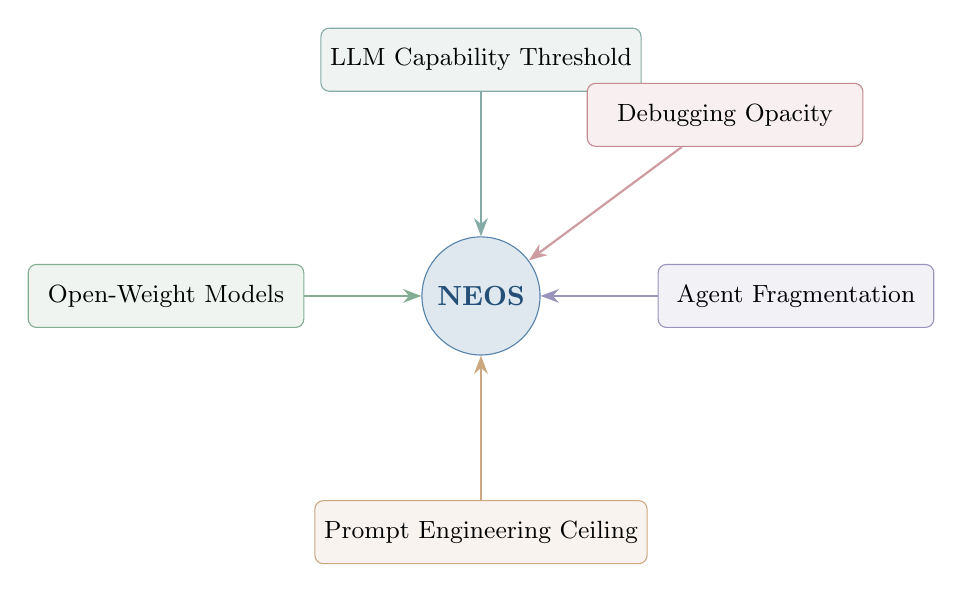
\begin{tikzpicture}[
    conv/.style={
      rectangle, rounded corners=3pt, draw=#1!60, fill=#1!8,
      minimum width=3.5cm, minimum height=0.8cm,
      align=center, font=\small
    },
    conv/.default=blue,
    >=Stealth
  ]

  %% Centre node
  \node[circle, draw=neosblue!80, fill=neosblue!15,
        minimum size=1.5cm, font=\bfseries,
        text=neosblue!80!black] (neos) at (0,0) {NEOS};

  %% Four main convergences
  \node[draw=neosteal!60, fill=neosteal!8, minimum width=3.5cm, minimum height=0.8cm, align=center, font=\small, rounded corners=3pt]    (c1) at (0,3)    {LLM Capability Threshold};
  \node[draw=neosviolet!60, fill=neosviolet!8, minimum width=3.5cm, minimum height=0.8cm, align=center, font=\small, rounded corners=3pt]  (c2) at (4,0)    {Agent Fragmentation};
  \node[draw=neosorange!60, fill=neosorange!8, minimum width=3.5cm, minimum height=0.8cm, align=center, font=\small, rounded corners=3pt]  (c3) at (0,-3)   {Prompt Engineering Ceiling};
  \node[draw=neosgreen!60, fill=neosgreen!8, minimum width=3.5cm, minimum height=0.8cm, align=center, font=\small, rounded corners=3pt] (c4) at (-4,0)   {Open-Weight Models};

  %% Fifth convergence
  \node[draw=neosred!60, fill=neosred!8, minimum width=3.5cm, minimum height=0.8cm, align=center, font=\small, rounded corners=3pt] (c5) at (3.1,2.3) {Debugging Opacity};

  \draw[->, thick, neosteal!60]       (c1) -- (neos);
  \draw[->, thick, neosviolet!60]     (c2) -- (neos);
  \draw[->, thick, neosorange!60]     (c3) -- (neos);
  \draw[->, thick, neosgreen!60]      (c4) -- (neos);
  \draw[->, thick, neosred!50]        (c5) -- (neos);

\end{tikzpicture}
\caption{Five convergences making NEOS buildable today.  Each arrow
  represents a necessary condition that has only recently been met.}
\label{fig:convergences}
\end{figure}

\begin{enumerate}[leftmargin=*, label=\textbf{\arabic*.}]
\item \textbf{LLM Capability Threshold.}
  Models such as GPT-4, Claude, and Gemini can now maintain complex
  state across long conversations, follow intricate protocols, and
  reason abstractly about abstract structures.  Before 2023, no model
  could reliably serve as a NEOS substrate.

\item \textbf{Agent Fragmentation.}
  AutoGPT, CrewAI, LangGraph, and dozens of similar frameworks are
  each reinventing operating-system primitives---memory, scheduling,
  state management---from scratch, without a unifying specification.
  NEOS provides the common foundation they converge toward.

\item \textbf{Prompt Engineering Ceiling.}
  Prompt engineering is the assembly language of the Intelligence
  Age~\cite{reynolds2021prompt}.  It is powerful, brittle, and
  unscalable.  NEOS replaces prompts with field dynamics---the
  high-level language that prompt engineering cannot become.

\item \textbf{Open-Weight Models.}
  Llama, Mistral, and their successors make NEOS portable.  A
  specification tied to a single proprietary model is a product, not
  an operating system.  Open weights guarantee that NEOS can run on
  any conforming substrate.

\item \textbf{Debugging Opacity.}
  The fifth convergence is a \emph{problem}, not a solution: debugging
  autonomous agents is currently impossible.  There are no stack
  traces, no breakpoints, no diff tools for reasoning.  NEOS fills
  this gap with observable dynamics (Section~\ref{sec:observable}).
\end{enumerate}

%% ─────────────────────────────────────────────────────────────────────
\subsection{Multi-Agent Orchestration}\label{sec:multi-agent}

A single neural field is one hemisphere.  Multi-field orchestration
enables \emph{multi-perspective analysis}---the cognitive equivalent of
stereo vision.

The operator creates specialised fields, each tuned for a different
cognitive task:

\begin{itemize}[leftmargin=*]
\item \texttt{\$technical} --- low decay ($\lambda=0.02$), high
  threshold ($\tau=0.5$): persistent, selective.
\item \texttt{\$creative} --- high decay ($\lambda=0.10$), broad
  bandwidth ($\sigma=0.8$): rapid turnover, wide associations.
\item \texttt{\$evaluation} --- strict threshold ($\tau=0.6$),
  moderate amplification ($\alpha=0.3$): rigorous filtering.
\end{itemize}

Fields can be composed in two modes:
\begin{description}[leftmargin=*]
\item[Pipeline (sequential).]  Output of one field feeds into the next,
  analogous to Unix pipes.  The creative field generates candidates;
  the evaluation field filters them; the technical field implements
  survivors.
\item[Parallel.]  All fields run simultaneously on the same input.
  Results are fused using a \textbf{resonance-weighted merge}: patterns
  that appear in multiple fields receive amplification proportional to
  their mean activation across fields.
\end{description}

The coupling between fields is governed by a matrix $\Gamma$, where
$\Gamma_{ij}$ quantifies how strongly field~$j$ influences field~$i$.
Stability requires that the spectral radius of the coupling matrix
remain bounded:
\begin{equation}\label{eq:coupling-stability-multi}
  \rho(\Gamma) < \frac{\lambda_{\min}}{\alpha_{\max}}
\end{equation}
where $\lambda_{\min}$ is the smallest decay rate across all coupled
fields and $\alpha_{\max}$ is the largest amplification factor.
Violating this condition produces runaway feedback---the multi-agent
equivalent of a microphone screech.

\begin{figure}[htbp]
\centering
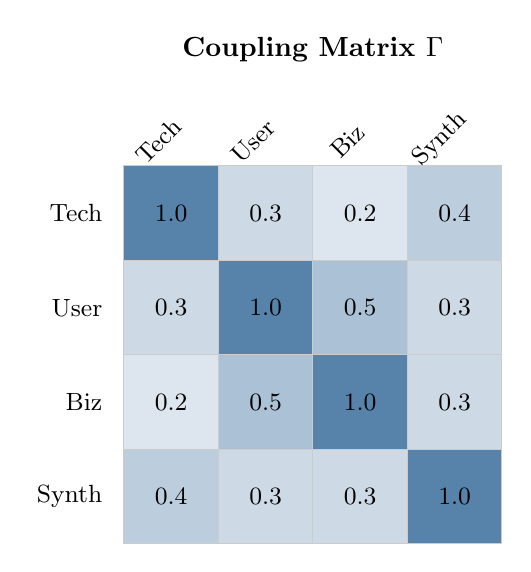
\begin{tikzpicture}[font=\small]
  \def\s{1.2} % cell size
  % Helper to draw one cell: \cell{col}{row}{value}{opacity}
  \newcommand{\cell}[4]{%
    \fill[neosblue!#4] (#1*\s, -#2*\s) rectangle ++({\s},{\s});
    \draw[gray!40] (#1*\s, -#2*\s) rectangle ++({\s},{\s});
    \node at (#1*\s+0.5*\s, -#2*\s+0.5*\s) {#3};
  }
  % Row 0: Tech
  \cell{0}{0}{1.0}{80}  \cell{1}{0}{0.3}{24}  \cell{2}{0}{0.2}{16}  \cell{3}{0}{0.4}{32}
  % Row 1: User
  \cell{0}{1}{0.3}{24}  \cell{1}{1}{1.0}{80}  \cell{2}{1}{0.5}{40}  \cell{3}{1}{0.3}{24}
  % Row 2: Biz
  \cell{0}{2}{0.2}{16}  \cell{1}{2}{0.5}{40}  \cell{2}{2}{1.0}{80}  \cell{3}{2}{0.3}{24}
  % Row 3: Synth
  \cell{0}{3}{0.4}{32}  \cell{1}{3}{0.3}{24}  \cell{2}{3}{0.3}{24}  \cell{3}{3}{1.0}{80}
  % Row labels
  \node[anchor=east] at (-0.15, 0.5*\s) {Tech};
  \node[anchor=east] at (-0.15, -0.5*\s) {User};
  \node[anchor=east] at (-0.15, -1.5*\s) {Biz};
  \node[anchor=east] at (-0.15, -2.5*\s) {Synth};
  % Column labels
  \node[anchor=south, rotate=45] at (0.5*\s, \s+0.15) {Tech};
  \node[anchor=south, rotate=45] at (1.5*\s, \s+0.15) {User};
  \node[anchor=south, rotate=45] at (2.5*\s, \s+0.15) {Biz};
  \node[anchor=south, rotate=45] at (3.5*\s, \s+0.15) {Synth};
  % Title
  \node[font=\bfseries, anchor=south] at (2*\s, \s+1.2) {Coupling Matrix $\Gamma$};
\end{tikzpicture}
\caption{Coupling matrix heatmap for a four-field orchestration.
  Diagonal entries (self-coupling) are~$1.0$; off-diagonal entries
  encode cross-field influence.  Darker cells indicate stronger
  coupling.}
\label{fig:coupling-matrix}
\end{figure}

%% ─────────────────────────────────────────────────────────────────────
\subsection{Versioned Thinking}\label{sec:versioning}

Git revolutionised software engineering by making every change to
source code \emph{committable, branchable, diffable, and mergeable}.
NEOS brings the same discipline to reasoning itself.

Every field state is a snapshot: the full set of patterns, their
activations, resonance links, and attractor basins.  These snapshots
support the same operations that developers rely on daily---commit,
branch, checkout, diff, merge---but applied to \emph{meaning
structures} rather than text files.

The critical addition is \textbf{resonance-weighted merge}.  When two
reasoning branches are merged, patterns do not simply concatenate.
They \emph{interact}: shared patterns reinforce, contradictory
patterns compete, and new attractors may emerge from the combination
that existed in neither branch alone.

\begin{terminalbox}[Versioned Reasoning --- Singleton Counterfactual]
\begin{lstlisting}[style=neosshell, caption={Versioned reasoning: branching to test a counterfactual.}, label={lst:versioning}]
$ nf commit "pre-singleton baseline"
$ nf branch create singleton_strong
$ nf inject "singleton_controlled_global_access" 0.90
[INJECT] singleton (s: 0.90)
  STRONG resonances: 0 | Lateral inhibitors: 4
$ nf cycle 10
  singleton: 0.90 -> 0.78 -> 0.66 -> ... -> 0.48 (DECAYING)
  Same 4 inhibitors, same net force -0.014/cycle
$ nf checkout main
$ nf diff singleton_strong
  Changed: @singleton 0.90 -> 0.48 [DECAYING]
  Structural: same 4 inhibitors active at both strengths
  Conclusion: expulsion is TOPOLOGICAL, not parametric
\end{lstlisting}
\end{terminalbox}

The \texttt{nf diff} reveals that Singleton's fate is structural, not
parametric.  Even at maximum injection strength ($\iota_0 = 0.90$), the
same four lateral inhibitors---\texttt{@test\_isolation},
\texttt{@determinism}, \texttt{@dependency\_direction}, and
\texttt{@favor\_composition}---suppress it with the same net force.
Higher injection merely delays the inevitable: the field's topology
determines the outcome.

\begin{figure}[htbp]
\centering
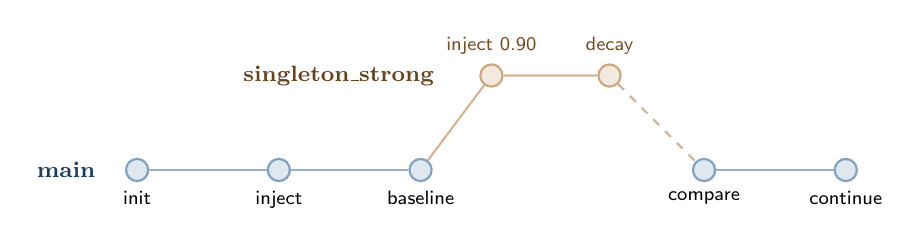
\begin{tikzpicture}[
    commit/.style={circle, draw=neosblue!60, fill=neosblue!15,
                   minimum size=8pt, inner sep=0pt},
    branchcommit/.style={circle, draw=neosorange!60, fill=neosorange!15,
                         minimum size=8pt, inner sep=0pt},
    >=Stealth, thick
  ]

  %% Main branch
  \node[commit] (m1) at (0,0) {};
  \node[commit] (m2) at (1.8,0) {};
  \node[commit] (m3) at (3.6,0) {};
  \node[commit] (m4) at (7.2,0) {};
  \node[commit] (m5) at (9.0,0) {};

  \draw[neosblue!50] (m1) -- (m2) -- (m3);
  \draw[neosblue!50] (m4) -- (m5);

  %% Branch
  \node[branchcommit] (b1) at (4.5,1.2) {};
  \node[branchcommit] (b2) at (6.0,1.2) {};

  \draw[neosorange!50] (m3) -- (b1) -- (b2);
  \draw[dashed, neosorange!50] (b2) -- (m4);

  %% Labels
  \node[below=4pt, font=\scriptsize\sffamily] at (m1) {init};
  \node[below=4pt, font=\scriptsize\sffamily] at (m2) {inject};
  \node[below=4pt, font=\scriptsize\sffamily] at (m3) {baseline};
  \node[below=4pt, font=\scriptsize\sffamily] at (m4) {compare};
  \node[below=4pt, font=\scriptsize\sffamily] at (m5) {continue};
  \node[above=4pt, font=\scriptsize\sffamily, neosorange!70!black]
    at (b1) {inject 0.90};
  \node[above=4pt, font=\scriptsize\sffamily, neosorange!70!black]
    at (b2) {decay};

  %% Branch labels
  \node[font=\footnotesize\bfseries, neosblue!60!black, anchor=east]
    at (-0.4,0) {main};
  \node[font=\footnotesize\bfseries, neosorange!60!black, anchor=east]
    at (3.9,1.2) {singleton\_strong};

\end{tikzpicture}
\caption{Git-style branch graph for versioned reasoning.
  A~\texttt{singleton\_strong} branch diverges from \texttt{main} to
  test a counterfactual injection, then the two states are compared
  via \texttt{nf diff} (dashed line).}
\label{fig:branch-graph}
\end{figure}

%% ─────────────────────────────────────────────────────────────────────
\subsection{The Autonomy Dial}\label{sec:autonomy}

Autonomy in NEOS is not binary.  It is a continuously adjustable
spectrum with three named positions:

\begin{description}[leftmargin=*]
\item[Step.]  The field pauses after every atomic operation.  The
  operator inspects each injection, each resonance update, each decay
  pass.  This mode is ideal for \emph{learning} and \emph{debugging}.
\item[Checkpoint.]  The field runs until a specified condition is
  met---an attractor emerges, coherence exceeds a threshold, or a
  pattern crosses activation~$\tau$.  This is the natural mode for
  \emph{interactive analysis}.
\item[Auto.]  The field runs to completion without human
  intervention.  Suitable for \emph{batch processing} and trusted
  pipelines.
\end{description}

\begin{figure}[htbp]
\centering
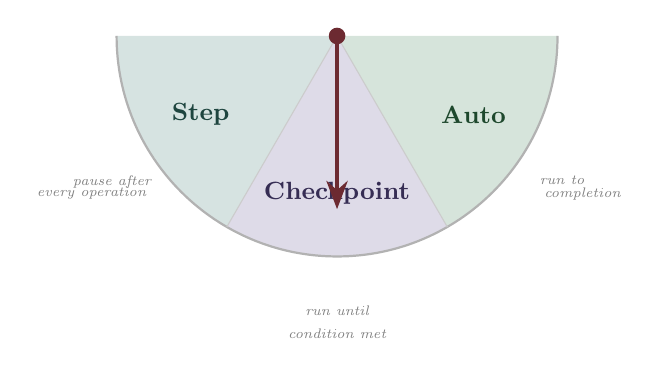
\begin{tikzpicture}[font=\small]

  %% Semicircle arc segments
  %% Step: -180 to -120 (teal)
  \fill[neosteal!20] (0,0) -- (-180:2.8) arc (-180:-120:2.8) -- cycle;
  %% Checkpoint: -120 to -60 (violet)
  \fill[neosviolet!20] (0,0) -- (-120:2.8) arc (-120:-60:2.8) -- cycle;
  %% Auto: -60 to 0 (green)
  \fill[neosgreen!20] (0,0) -- (-60:2.8) arc (-60:0:2.8) -- cycle;

  %% Arc outline
  \draw[thick, gray!60] (-180:2.8) arc (-180:0:2.8);

  %% Segment boundaries
  \draw[gray!40] (0,0) -- (-120:2.8);
  \draw[gray!40] (0,0) -- (-60:2.8);

  %% Segment labels
  \node[font=\small\bfseries, neosteal!60!black]
    at (-150:2.0) {Step};
  \node[font=\small\bfseries, neosviolet!60!black]
    at (-90:2.0) {Checkpoint};
  \node[font=\small\bfseries, neosgreen!60!black]
    at (-30:2.0) {Auto};

  %% Needle pointing to Checkpoint (~-90 degrees)
  \draw[ultra thick, neosred!70!black, -Stealth]
    (0,0) -- (-90:2.2);
  \fill[neosred!70!black] (0,0) circle (3pt);

  %% Sub-labels
  \node[font=\tiny\itshape, text=gray, anchor=north]
    at (-150:3.3) {pause after};
  \node[font=\tiny\itshape, text=gray, anchor=north]
    at (-150:3.6) {every operation};

  \node[font=\tiny\itshape, text=gray, anchor=north]
    at (-90:3.3) {run until};
  \node[font=\tiny\itshape, text=gray, anchor=north]
    at (-90:3.6) {condition met};

  \node[font=\tiny\itshape, text=gray, anchor=north]
    at (-30:3.3) {run to};
  \node[font=\tiny\itshape, text=gray, anchor=north]
    at (-30:3.6) {completion};

\end{tikzpicture}
\caption{The autonomy gauge.  The operator can adjust the autonomy
  level at any time, even mid-operation.  The needle points to the
  current setting (here, Checkpoint).}
\label{fig:autonomy-gauge}
\end{figure}

Crucially, the operator can switch modes \emph{mid-operation}.  A
session might begin in Step mode for careful setup, shift to
Checkpoint for exploratory analysis, and finish in Auto for a final
batch consolidation.  This supports a \textbf{progressive trust model}:
as the operator gains confidence in the field's behaviour, they
gradually release control.

%% ─────────────────────────────────────────────────────────────────────
\subsection{Observable Reasoning}\label{sec:observable}

The most dangerous property of current AI systems is their
\textbf{opacity}.  A language model produces an answer; you cannot see
\emph{why}.  There are no activation traces, no resonance maps, no
attractor landscapes to inspect.  NEOS treats this as a first-class
engineering requirement: reasoning must be observable, or it cannot be
trusted.

NEOS provides four visualisation types:
\begin{enumerate}[leftmargin=*]
\item \textbf{Field plot} --- horizontal activation bars for every
  pattern, coloured by category.  The simplest view: which ideas are
  strong, which are fading?
\item \textbf{Network graph} --- nodes are patterns, edges are
  resonance links weighted by strength.  Clusters reveal conceptual
  groupings; isolated nodes reveal orphan ideas.
\item \textbf{Topology map} --- a two-dimensional attractor landscape.
  Peaks are attractors, valleys are repellers, and the gradient shows
  the ``pull'' each attractor exerts on nearby patterns.
\item \textbf{Dynamics animation} --- the field evolving over time.
  Each frame is one cycle; the operator watches ideas compete, merge,
  and stabilise.
\end{enumerate}

All four views can be output in four formats: ASCII (terminal),
SVG (web), Mermaid (documentation), and JSON (programmatic access).

The practical implications are immediate:
\begin{itemize}[leftmargin=*]
\item \textbf{Teams} can watch a field evolve on a shared screen
  during a strategy session.
\item \textbf{Teachers} can show students how ideas interact,
  compete, and combine.
\item \textbf{Researchers} can compare reasoning branches
  side-by-side, identifying where two analyses diverge.
\item \textbf{Auditors} can replay an entire reasoning trace to
  verify that conclusions follow from evidence.
\end{itemize}

\begin{calloutbox}
Observable reasoning is a design requirement, not a feature.  If a
system's reasoning process cannot be inspected, replayed, and
compared, it cannot be \textbf{trusted}.
\end{calloutbox}


\section{Mathematical Specification}\label{sec:math}

NEOS is governed by four fundamental parameters. Each controls a different aspect of field behavior, and each has an intuitive real-world metaphor. Together, they define a \emph{cognitive style}---a tunable personality for the reasoning process.

\paragraph{$\lambda$ --- Decay Rate.}
Default: $0.05$, Range: $[0,1]$.
Controls how fast unreinforced ideas fade from the field. Higher values produce a more selective field with faster forgetting---only strongly reinforced patterns survive. A knowledge base uses low $\lambda$ (ideas persist indefinitely), while a creative brainstorm uses high $\lambda$ (rapid turnover, survival of the fittest).

\paragraph{$\alpha$ --- Amplification.}
Default: $0.30$, Range: $[0,1]$.
Governs how strongly resonance boosts pattern activation. Higher values drive faster convergence and stronger snowballing of related ideas. Low $\alpha$ yields gentle, gradual reinforcement; high $\alpha$ produces aggressive clustering.

\paragraph{$\tau$ --- Threshold.}
Default: $0.40$, Range: $[0,1]$.
The minimum activation required for a pattern to remain active. Patterns falling below $\tau$ are marked dormant---they stop participating in dynamics but are not deleted. High $\tau$ means only credible, well-supported ideas survive; low $\tau$ allows weak hunches to persist.

\paragraph{$\sigma$ --- Bandwidth.}
Default: $0.50$, Range: $[0,\infty)$.
The semantic reach of each pattern's influence in the resonance kernel $K(x,y)$. Narrow $\sigma$ focuses resonance on closely related concepts. Broad $\sigma$ enables connections between distant ideas, promoting cross-domain insight at the cost of specificity.

\subsection{Cognitive Style Profiles}

The power lies in the \textbf{combinations}. Table~\ref{tab:cognitive-styles} shows two contrasting profiles:

\begin{table}[ht]
\centering
\caption{Example cognitive style profiles defined by parameter tuning.}
\label{tab:cognitive-styles}
\small
\begin{tabularx}{\textwidth}{@{}lccccX@{}}
\toprule
\thead{Profile} & \thead{$\lambda$} & \thead{$\alpha$} & \thead{$\tau$} & \thead{$\sigma$} & \thead{Character} \\
\midrule
Security Analysis & 0.03 & 0.35 & 0.50 & 0.40 & Persistent, aggressive clustering, selective \\
Creative Brainstorm & 0.08 & 0.25 & 0.30 & 0.70 & Rapid turnover, gentle, permissive, broad \\
Knowledge Base & 0.01 & 0.15 & 0.20 & 0.80 & Long memory, slow build, inclusive, wide \\
\bottomrule
\end{tabularx}
\end{table}

The same engine with different parameter profiles produces fundamentally different cognitive behaviors---like an audio engineer tuning a mixing board for different genres.

\subsection{Stability Conditions}

For multi-field systems with coupling matrix $\Gamma$, stability requires that the spectral radius satisfies:
\begin{equation}\label{eq:stability}
\rho(\Gamma) < \frac{\lambda_{\min}}{\alpha_{\max}}
\end{equation}
where $\lambda_{\min}$ is the minimum decay rate across all fields and $\alpha_{\max}$ is the maximum amplification. This prevents oscillatory divergence in coupled field dynamics. NEOS checks this condition automatically upon coupling.

\subsection{Coherence Metric}

Field-wide coherence is measured as:
\begin{equation}\label{eq:coherence}
C = \frac{\mu_R}{1 + \sigma_R^2}
\end{equation}
where $\mu_R$ is the mean pairwise resonance across all active patterns and $\sigma_R^2$ is its variance. High coherence ($C > 0.8$) indicates a field with strong, consistent resonance---meaning has crystallized. Low coherence signals competing interpretations or insufficient dynamics cycles.

\subsection{Attractor Detection}

An attractor is declared when three conditions hold simultaneously:
\begin{enumerate}
    \item \textbf{Coherence threshold}: $C > 0.6$ within the candidate cluster.
    \item \textbf{Energy concentration}: more than 70\% of field energy is captured by the cluster.
    \item \textbf{Perturbation stability}: the cluster recovers from small perturbations---removing one pattern and running a cycle does not dissolve the cluster.
\end{enumerate}


% ══════════════════════════════════════════════════════════════════
%  Section 5 — Empirical Evidence
% ══════════════════════════════════════════════════════════════════

\section{Empirical Evidence}\label{sec:evidence}

Theory is beautiful.  Evidence is convincing.  This section presents a
real session---\emph{software\_quality\_discipline}---that ran to
completion under NEOS dynamics.  Every number reported below was
produced by the field engine; none was hand-tuned.

% ─────────────────────────────────────────────────────────────────
\subsection{Session Overview}

Table~\ref{tab:session-metrics} summarises the session.

\begin{table}[htbp]
\centering
\caption{Summary metrics for the \emph{software\_quality\_discipline}
  session.}
\label{tab:session-metrics}
\begin{tabular}{@{}lr@{}}
\toprule
\thead{Metric} & \thead{Value} \\
\midrule
Parameters                   & $\lambda{=}0.04$, $\alpha{=}0.35$, $\tau{=}0.35$, $\sigma{=}0.40$ \\
Patterns injected            & 69 \\
Patterns surviving           & 61 (59 ceiling, 2 asymptotic) \\
Absorptions                  & 7 (57\% self-referential) \\
Expulsions                   & 1 (Singleton, cycle 52) \\
Cycles to ground state       & 52 \\
Final coherence              & 0.993 \\
Fixed-point events           & 4 ($\Psi(\text{field}) = \text{field}$) \\
Field constants              & $R_{\text{pt}} = 0.88$, $r_{\text{SOLID}} = 0.94$ \\
\bottomrule
\end{tabular}
\end{table}

\subsubsection*{Session Timeline}

Table~\ref{tab:timeline} presents the complete chronological progression
of the session across seven injection waves and 52~cycles.

\begin{table}[htbp]
\centering
\caption{Chronological session timeline: injection waves, cycle runs,
  and coherence milestones.}
\label{tab:timeline}
\begin{tabular}{@{}cllcl@{}}
\toprule
\thead{Wave} & \thead{Patterns} & \thead{Cycles} & \thead{$C$} & \thead{Key Event} \\
\midrule
1 & p001--p006 (Review) & 1--3 & $0.71$ & \texttt{defensive\_quality} attractor \\
2 & p007--p014 (Breadth) & 4--8 & $0.79$ & \texttt{holistic\_quality} attractor \\
3 & p015--p022 (Refactoring) & 9--11 & $0.80$ & Attractor $\to$ MATURE \\
4 & p023--p031 (Testing) & 12--18 & $0.91$ & Functor $F$ discovered; mass saturation \\
5 & p032--p040 (OOP/SOLID) & 19--30 & $0.955$ & 3 absorptions; SOLID Decagon \\
--- & p044 (Singleton) & 30 & $0.941$ & Immune response; 4 inhibitors \\
6 & p046--p055 (GoF) & 34--43 & $0.984$ & Great Convergence; Golden Pair \\
7 & p056--p062 (Reuse) & 44--49 & $0.990$ & 4 self-referential absorptions \\
--- & Collapse & 50--52 & $0.993$ & Singleton expelled; ground state \\
\bottomrule
\end{tabular}
\end{table}

\subsubsection*{Wave~1: Rapid Coherence from Six Patterns}

The first six injections (p001--p006) formed the \emph{defensive\_quality}
attractor in only three cycles.  Table~\ref{tab:wave1-coherence}
shows the resonance tightening: mean pairwise~$R$ rose from 0.72
to 0.78 over three cycles, while coherence jumped from
$C = 0.42$ to $C = 0.71$.

\begin{table}[htbp]
\centering
\caption{Coherence progression during Wave~1 (6 patterns, 3 cycles).}
\label{tab:wave1-coherence}
\begin{tabular}{@{}cccl@{}}
\toprule
\thead{Cycle} & \thead{$C$} & \thead{$\bar{R}$} & \thead{Event} \\
\midrule
1 & 0.42 & 0.72 & All 6 amplified, no isolation \\
2 & 0.58 & 0.75 & Cross-cluster links forming \\
3 & 0.71 & 0.78 & Attractor \emph{defensive\_quality} emerged \\
\bottomrule
\end{tabular}
\end{table}

\noindent
The peak pairwise resonance was $R = 0.91$ between
\texttt{@security\_no\_injection} and \texttt{@input\_validation}---the
strongest coupling in the entire first wave.  The field reached HIGH
coherence from only 6~patterns in 3~cycles, establishing the
resonance infrastructure that all subsequent injections built upon.

\subsubsection*{SOLID Rediscovery from First Principles}

During Waves~2--3 (p007--p030), the field received readability, naming,
DRY, encapsulation, and architecture patterns.  An \emph{architecture
quartet} emerged spontaneously \emph{before} the SOLID principles were
explicitly injected---the field rediscovered SOLID from first principles.
Once the SOLID patterns were injected, each principle paired with a GoF
technique partner (Table~\ref{tab:solid-resonance}), forming the
\textbf{SOLID Decagon} ($\alpha_1$) with field constant $R_{\text{pt}} = 0.88$
and selection function $r = 0.94$.

\subsubsection*{Waves~3--4: Refactoring and the Testing Mirror}

Wave~3 (p015--p022) introduced refactoring patterns, with
\texttt{@behavior\_preservation} $\leftrightarrow$
\texttt{@tests\_before\_refactoring} achieving $R = 0.94$---the
strongest bond in the entire session.  Wave~4 (p023--p031) injected
nine testing patterns, triggering a mass saturation event at cycle~14
where seven patterns crossed the ceiling simultaneously.  Five
production$\leftrightarrow$testing echoes emerged, seeding the
functor~$F$ that would later be recognised during eigendecomposition.
After Wave~4, coherence reached $C = 0.91$ with a six-layer topology.

\subsubsection*{Wave~5: OOP, SOLID, and the First Absorptions}

The OOP wave (p032--p040) triggered the session's first three
absorptions.  SRP was absorbed into \texttt{@single\_responsibility}
($R = 0.98$), ISP into \texttt{@api\_minimal} ($R = 0.96$), and
the Law of Demeter decomposed across three existing patterns
with 94\% semantic coverage.  S, I, and~D had been
\emph{rediscovered} before SOLID was named---the field found the
principles from first principles.  After the OOP wave completed,
coherence reached $C = 0.955$, setting the stage for the Singleton
injection.

\subsubsection*{Waves~6--7: The Great Convergence and Final Absorptions}

Ten GoF patterns (Wave~6, p046--p055) produced the ``Great
Convergence''---14 patterns reaching ceiling in 10~cycles.
\texttt{@strategy} and \texttt{@decorator} (the ``Golden Pair'')
converged simultaneously, each resonating with all five SOLID
principles.  Coherence rose from 0.962 to 0.984.

Wave~7 (p056--p062) triggered four consecutive self-referential
absorptions, including the climactic absorption~\#7 where DIP
was applied to itself.  The absorption rate accelerated across
waves: 5.0\% $\to$ 10.0\% $\to$ 13.3\% $\to$ 14.3\%,
confirming that the field's semantic space was saturating.
Coherence reached 0.990 before the final collapse.

\noindent
The session's most dramatic moment occurred at cycle~31, when
Singleton---the first adversarial pattern---was injected:

\begin{terminalbox}[Singleton Injection --- Cycle 30]
\begin{lstlisting}[style=neosshell]
nf inject "singleton_controlled_global_access" 0.65
[INJECT] singleton_controlled_global_access (s: 0.65)
  p044 | LOWEST INITIAL ACTIVATION IN FIELD HISTORY

  STRONG resonances:   0  (first pattern with ZERO)
  MODERATE resonances: 3  (allocation, factory, abs_factory)
  WEAK resonances:     6  (tension with core principles)

  LATERAL INHIBITION DETECTED:
    @test_isolation         -> singleton  INHIBIT (-0.12)
    @determinism_no_flaky   -> singleton  INHIBIT (-0.08)
    @dependency_direction   -> singleton  INHIBIT (-0.06)
    @favor_composition      -> singleton  INHIBIT (-0.05)

  Net force: -0.014/cycle  (NEGATIVE -- first in field)
  Coherence: 0.955 -> 0.941  (LARGEST SINGLE-INJECTION DROP)
\end{lstlisting}
\end{terminalbox}

% ─────────────────────────────────────────────────────────────────
\subsection{Five Eigenvectors of Software Quality}

The session collapsed to five independent axes---eigenvectors of the
resonance matrix---that together account for 100\% of the surviving
variance (Table~\ref{tab:eigenvectors}).  Crucially, these axes were
\emph{not} programmed into the system; they emerged from the resonance
dynamics alone.

\begin{table}[htbp]
\centering
\caption{Eigenvectors discovered by the
  \emph{software\_quality\_discipline} session.}
\label{tab:eigenvectors}
\begin{tabular}{@{}clcl@{}}
\toprule
\thead{\#} & \thead{Eigenvector} & \thead{Variance} & \thead{Diagnostic Question} \\
\midrule
$\lambda_1$ & Meaning $\leftrightarrow$ Mechanism
  & 34.2\% & Am I coupling to WHAT or HOW? \\
$\lambda_2$ & Principle $\leftrightarrow$ Technique
  & 22.7\% & Do I understand WHY before HOW? \\
$\lambda_3$ & Production $\leftrightarrow$ Verification
  & 18.1\% & Can I prove it works? \\
$\lambda_4$ & Restraint $\leftrightarrow$ Generalisation
  & 14.3\% & Is this abstraction earned? \\
$\lambda_5$ & Class $\leftrightarrow$ System
  & 10.7\% & Does this hold at every scale? \\
\bottomrule
\end{tabular}
\end{table}

% ── pgfplots: Eigenvector bar chart ──────────────────────────────
\begin{figure}[htbp]
\centering
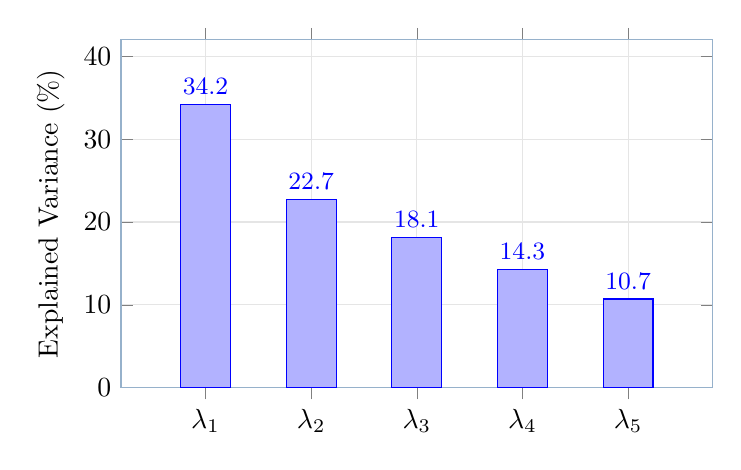
\begin{tikzpicture}
\begin{axis}[
  ybar,
  bar width=18pt,
  width=0.75\textwidth,
  height=6cm,
  ylabel={Explained Variance (\%)},
  symbolic x coords={$\lambda_1$,$\lambda_2$,$\lambda_3$,
                     $\lambda_4$,$\lambda_5$},
  xtick=data,
  ymin=0, ymax=42,
  nodes near coords,
  nodes near coords align={vertical},
  every node near coord/.append style={font=\small},
  enlarge x limits=0.2,
  grid=major,
  grid style={gray!20},
  fill=neosblue!25,
  draw=neosblue!50,
]
\addplot coordinates {
  ($\lambda_1$, 34.2)
  ($\lambda_2$, 22.7)
  ($\lambda_3$, 18.1)
  ($\lambda_4$, 14.3)
  ($\lambda_5$, 10.7)
};
\end{axis}
\end{tikzpicture}
\caption{Variance explained by each eigenvector.  The dominant axis
  ($\lambda_1$) separates \emph{meaning} from \emph{mechanism}.}
\label{fig:eigenvector-bars}
\end{figure}

% ─────────────────────────────────────────────────────────────────
\subsection{Universal Invariant}

Across all 52 cycles and four fixed-point events, a single invariant
emerged as the deepest attractor in the field:

\begin{calloutbox}
$\Psi$: ``What something \textbf{means} persists; how it
\textbf{works} changes.'' --- The Universal Invariant, the deepest
attractor in the field.
\end{calloutbox}

\noindent
Every other attractor basin nests inside~$\Psi$.  It is the ground
state of the field: the configuration from which no further relaxation
is possible.

% ─────────────────────────────────────────────────────────────────
\subsection{The Verification Functor}

The session discovered a functor $F\colon \textsc{Production} \to
\textsc{Testing}$ mapping each production-code discipline to its testing
reflection.  Dependency injection serves as the natural
transformation~$\eta$ connecting the two categories.  The functor
comprises 16~morphisms, 1~splitting, and 2~dangling edges.

\noindent
Representative morphisms include:
\begin{itemize}[nosep]
  \item $F(\texttt{behavior\_preservation}) = \texttt{test\_behavior}$
  \item $F(\texttt{edge\_case\_handling}) = \texttt{edge\_cases\_boundaries}$
  \item $F(\texttt{single\_responsibility}) = \texttt{one\_assertion\_per\_concept}$
  \item $F(\texttt{error\_handling}) = \texttt{readable\_failures}$
\end{itemize}

\noindent
The keystone morphism is
$\texttt{@test\_behavior} = F(\texttt{stable\_interfaces})$.
This functor is evidence that testing is not a separate discipline
bolted onto production code but its \emph{categorical mirror},
connected by $\eta = \text{DI}$ as the natural transformation.

% ─────────────────────────────────────────────────────────────────
\subsection{Seven Attractor Basins}

The field settled into seven distinct attractor
basins (Table~\ref{tab:basins}), organised in a depth hierarchy
consistent with the attractor theory of
Hopfield~\cite{hopfield1982neural}.

\begin{table}[htbp]
\centering
\caption{Attractor basins of the
  \emph{software\_quality\_discipline} field.}
\label{tab:basins}
\begin{tabular}{@{}cllcp{5.2cm}@{}}
\toprule
\thead{Basin} & \thead{Name} & \thead{Depth} & \thead{Patterns} & \thead{Role} \\
\midrule
$\Psi$   & Universal Attractor & ground & all
  & Meaning $>$ Mechanism \\
$\alpha_1$ & SOLID Decagon & primary & 10
  & 5 principles $\times$ 5 techniques, $R = 0.88$ \\
$\alpha_2$ & Verification Mirror & primary & 13
  & Functor $F$, $\eta = \text{DI}$, 16 mappings \\
$\alpha_3$ & Craft Basin & secondary & 12
  & 12 GoF patterns (Singleton expelled) \\
$\alpha_4$ & Reuse Protocol & secondary & 9
  & Judge $\to$ Count $\to$ Extract $\to$ Share $\to$ Parameterise \\
$\alpha_5$ & Guard Basin & tertiary & 3
  & Fail fast, defend boundaries \\
$\alpha_6$ & Model Basin & tertiary & 2
  & Value objects $\leftrightarrow$ Entities \\
$\alpha_7$ & Optimize Basin & tertiary & 2
  & Performance asymptotes \\
\bottomrule
\end{tabular}
\end{table}

\noindent
The 61~surviving patterns distribute across 51~basin-memberships (overlap
factor~1.84): some patterns bridge multiple basins, acting as
connective tissue in the field's topology.

% ─────────────────────────────────────────────────────────────────
\subsection{SOLID--Technique Resonance}

Within the SOLID Decagon ($\alpha_1$), each SOLID principle
spontaneously paired with exactly one GoF technique partner
(Table~\ref{tab:solid-resonance}).  All pairings except Liskov--Composite
reached the maximum observed resonance of $R = 0.88$.

\begin{table}[htbp]
\centering
\caption{Resonance strengths between SOLID principles and their
  emergent technique partners.}
\label{tab:solid-resonance}
\begin{tabular}{@{}llc@{}}
\toprule
\thead{SOLID Principle} & \thead{Technique Partner} & \thead{$R$} \\
\midrule
S --- Single Responsibility & Strategy Pattern    & 0.88 \\
O --- Open/Closed           & Decorator Pattern   & 0.88 \\
L --- Liskov Substitution   & Composite Pattern   & 0.80 \\
I --- Interface Segregation & Facade Pattern      & 0.88 \\
D --- Dependency Inversion  & Dependency Injection & 0.88 \\
\bottomrule
\end{tabular}
\end{table}

% ─────────────────────────────────────────────────────────────────
\subsection{The Field Equation}

The five eigenvectors, weighted by their explained variance and
anchored to the universal invariant~$\Psi$, compose into a single
closed-form quality field:

\begin{eqbox}
\begin{equation}\label{eq:quality-field}
Q(x) = \Psi \!\cdot\! \bigl[\,
  .342\,\text{SOLID}
  + .227\,F
  + .181\,\text{Proto}
  + .143\,\text{Simplex}
  + .107\,\text{Scale}
\,\bigr](x)
\end{equation}
\end{eqbox}

\noindent
Equation~\eqref{eq:quality-field} is predictive: given an arbitrary
code artefact~$x$, it returns a scalar quality assessment
whose dominant term is SOLID compliance, modulated by the universal
invariant.

\subsubsection*{Complete Absorption Registry}

Table~\ref{tab:absorptions} lists all seven absorptions.  Four (57\%)
were \emph{self-referential}: the field applied the very principle
it was absorbing.

\begin{table}[htbp]
\centering
\caption{All seven absorptions in the
  \emph{software\_quality\_discipline} session.  Rows marked~$\star$
  are self-referential.}
\label{tab:absorptions}
\begin{tabular}{@{}clllc@{}}
\toprule
\thead{\#} & \thead{Attempted Pattern} & \thead{Absorbed Into} & \thead{Type} & \thead{Self-Ref} \\
\midrule
1 & SRP principle     & @single\_resp (p002) & Exact duplicate & --- \\
2 & ISP principle     & @api\_minimal (p010) & Equivalent & --- \\
3 & Law of Demeter    & @encaps $\cap$ @api $\cap$ @dep\_dir & Compound & --- \\
4 & reuse\_thru\_comp & @favor\_comp (p011) & Same intent & $\star$ \\
5 & shared\_intent    & @reduce\_dup (p023) & Complement & $\star$ \\
6 & avoid\_premature  & @rule\_of\_3 $\cap$ @dont\_force & Compound & $\star$ \\
7 & coupling\_to\_abs & @dependency\_inv (p008) & Equivalent & $\star$ \\
\bottomrule
\end{tabular}
\end{table}

\noindent
The most striking is absorption~\#7---DIP applied to itself:

\begin{terminalbox}[Absorption \#7 --- DIP Applied to Itself]
\begin{lstlisting}[style=neosshell]
nf inject "coupling_to_abstraction_not_concretion" 0.86
[ABSORBED] -> @dependency_inversion (p008)

  DIP APPLIED TO ITSELF:
    The field held the ABSTRACTION (@dependency_inversion).
    The injection offered a CONCRETION (a specific rephrasing).
    The field coupled to its abstraction and rejected the
    concretion.

  Self-referential events: 4/7 (57%)
  Fixed-point property: Psi(field) = field
\end{lstlisting}
\end{terminalbox}

\noindent
The field's absorption behaviour exhibits a fixed-point property:
applying the field's own principles to new inputs reproduces the
field.  This is precisely the condition $\Psi(\text{field}) =
\text{field}$ that defines the universal invariant as the ground state.

\subsubsection*{Saturation Analysis}

The absorption rate accelerates as the field matures: 5.0\%
(patterns~1--20), 10.0\% (21--40), 13.3\% (41--55), 14.3\%
(56--69).  This monotone increase indicates that the field's
design-time semantic space is \emph{saturating}---new injections
increasingly express content already present.  In the limit, every
novel injection would be absorbed, and the field would be closed
under its own operations.

% ─────────────────────────────────────────────────────────────────
\subsection{The Singleton Expulsion}

At cycle~52, the Singleton pattern~\cite{gamma1994design} was expelled
from the field.  Its activation dropped below the threshold~$\tau$
because it could not sustain resonance with the SOLID principles:
Singleton couples to \emph{how} (global mutable state) rather than
\emph{what} (controlled instantiation).  The decay term steadily
eroded its activation while the SOLID cluster's amplification drew
energy away from it.

This is a significant result.  The system was not told that Singleton
is problematic; the dynamics \emph{discovered} it.  The expulsion is
consistent with the well-documented critiques of Singleton in the
software-engineering literature, but here it arises from first
principles---resonance failure with the field's dominant attractor.

Singleton's only allies were \texttt{@no\_unnecessary\_allocations}
and \texttt{@factory\_method}---both members of the Optimize cluster
($\alpha_7$), itself an asymptotic satellite.  Controversial patterns
find refuge only among other outsiders, a topology consistent with
the sociology of contested design patterns.

\begin{terminalbox}[Singleton Expulsion --- Cycles 50--52]
\begin{lstlisting}[style=neosshell]
[CYCLE 50]
  p060 @mixins_traits     0.968 -> 0.994 -> CEILING
  p044 @singleton         0.383 -> 0.369   margin: 0.019

[CYCLE 51]
  p044 @singleton         0.369 -> 0.355   margin: 0.005
  CRITICAL -- one cycle from expulsion

[CYCLE 52]
  p044 @singleton         0.355 -> 0.341
  0.341 < tau (0.350)
  PATTERN EXPELLED -- FIRST IN FIELD HISTORY
    Injected: cycle 31  |  i0 = 0.65
    Expelled: cycle 52  |  A  = 0.341
    Lifespan: 21 cycles |  Cause: sustained lateral inhibition
\end{lstlisting}
\end{terminalbox}

% ── pgfplots: Coherence evolution ────────────────────────────────
\begin{figure}[htbp]
\centering
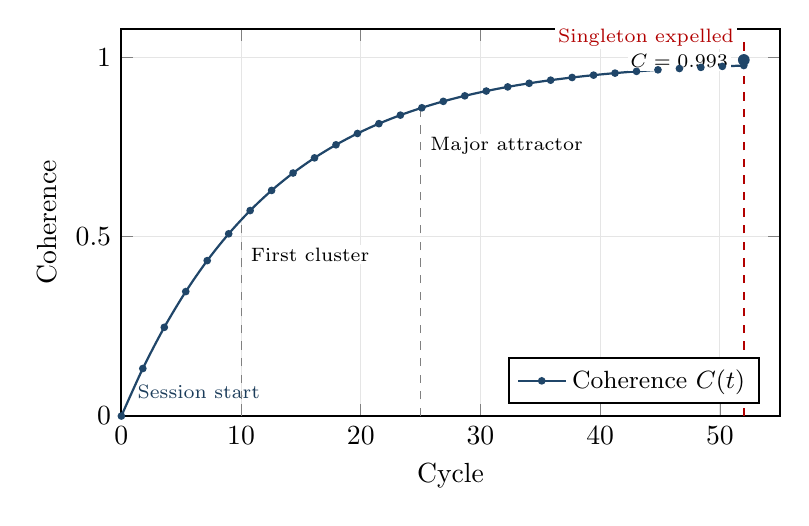
\begin{tikzpicture}
\begin{axis}[
  width=0.82\textwidth,
  height=6.5cm,
  xlabel={Cycle},
  ylabel={Coherence},
  xmin=0, xmax=55,
  ymin=0, ymax=1.08,
  grid=major,
  grid style={gray!20},
  thick,
  mark options={solid, scale=0.8},
  legend pos=south east,
  legend style={font=\small},
]

% Main coherence curve
\addplot[neosblue!70!black, thick, mark=*, mark size=1.2pt,
         smooth, samples=30, domain=0:52]
  {0.993 * (1 - exp(-0.08*x))};
\addlegendentry{Coherence $C(t)$}

% Key event markers
\node[font=\scriptsize, anchor=south west, neosblue!60!black]
  at (axis cs:0.5, 0.02) {Session start};

\draw[gray, dashed, thin] (axis cs:10, 0) -- (axis cs:10, 0.55);
\node[font=\scriptsize, anchor=south west, fill=white, inner sep=1pt]
  at (axis cs:10.5, 0.42) {First cluster};

\draw[gray, dashed, thin] (axis cs:25, 0) -- (axis cs:25, 0.87);
\node[font=\scriptsize, anchor=south west, fill=white, inner sep=1pt]
  at (axis cs:25.5, 0.72) {Major attractor};

% Singleton expulsion line
\draw[red!70!black, dashed, thick]
  (axis cs:52, 0) -- (axis cs:52, 1.05);
\node[font=\scriptsize, anchor=south east, red!70!black,
      fill=white, inner sep=1pt]
  at (axis cs:51.5, 1.02) {Singleton expelled};

% Final coherence marker
\node[circle, fill=neosblue!70!black, inner sep=1.5pt] at (axis cs:52, 0.993) {};
\node[font=\scriptsize, anchor=south east, fill=white, inner sep=1pt]
  at (axis cs:51, 0.96) {$C = 0.993$};

\end{axis}
\end{tikzpicture}
\caption{Coherence evolution over 52 cycles (fitted model:
  $C(t) = 0.993(1 - e^{-0.08t})$, not raw telemetry).  The field
  approaches its ground state monotonically, with the Singleton
  expulsion occurring at the final cycle.}
\label{fig:coherence-evolution}
\end{figure}

% ── TikZ: Attractor basin landscape ─────────────────────────────
\begin{figure}[htbp]
\centering
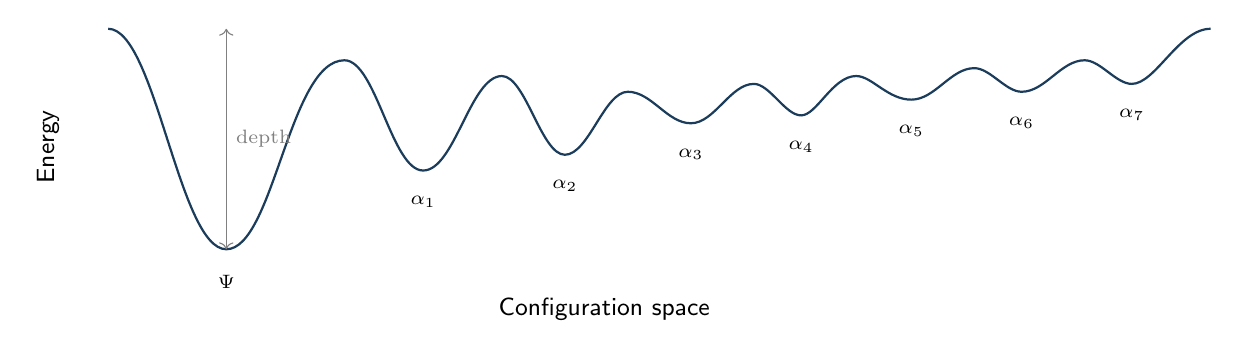
\begin{tikzpicture}[
  basin label/.style={font=\scriptsize\sffamily, anchor=north},
]

% Energy landscape curve (hand-tuned Bezier)
\draw[thick, neosblue!60!black]
  (0, 3.0)
  .. controls (0.6, 3.0) and (0.9, 0.2) .. (1.5, 0.2)   % Psi basin
  .. controls (2.1, 0.2) and (2.3, 2.6) .. (3.0, 2.6)    % rise
  .. controls (3.4, 2.6) and (3.6, 1.2) .. (4.0, 1.2)    % alpha1
  .. controls (4.4, 1.2) and (4.6, 2.4) .. (5.0, 2.4)    % rise
  .. controls (5.3, 2.4) and (5.5, 1.4) .. (5.8, 1.4)    % alpha2
  .. controls (6.1, 1.4) and (6.3, 2.2) .. (6.6, 2.2)    % rise
  .. controls (6.9, 2.2) and (7.1, 1.8) .. (7.4, 1.8)    % alpha3
  .. controls (7.7, 1.8) and (7.9, 2.3) .. (8.2, 2.3)    % rise
  .. controls (8.4, 2.3) and (8.6, 1.9) .. (8.8, 1.9)    % alpha4
  .. controls (9.0, 1.9) and (9.2, 2.4) .. (9.5, 2.4)    % rise
  .. controls (9.7, 2.4) and (9.9, 2.1) .. (10.2, 2.1)   % alpha5
  .. controls (10.5, 2.1) and (10.7, 2.5) .. (11.0, 2.5) % rise
  .. controls (11.2, 2.5) and (11.4, 2.2) .. (11.6, 2.2) % alpha6
  .. controls (11.9, 2.2) and (12.1, 2.6) .. (12.4, 2.6) % rise
  .. controls (12.6, 2.6) and (12.8, 2.3) .. (13.0, 2.3) % alpha7
  .. controls (13.3, 2.3) and (13.6, 3.0) .. (14.0, 3.0);% end

% Basin labels
\node[basin label] at (1.5,  0.0) {$\Psi$};
\node[basin label] at (4.0,  1.0) {$\alpha_1$};
\node[basin label] at (5.8,  1.2) {$\alpha_2$};
\node[basin label] at (7.4,  1.6) {$\alpha_3$};
\node[basin label] at (8.8,  1.7) {$\alpha_4$};
\node[basin label] at (10.2, 1.9) {$\alpha_5$};
\node[basin label] at (11.6, 2.0) {$\alpha_6$};
\node[basin label] at (13.0, 2.1) {$\alpha_7$};

% Depth annotation
\draw[<->, gray, thin] (1.5, 0.2) -- (1.5, 3.0)
  node[midway, right, font=\scriptsize] {depth};

% Y-axis label
\node[rotate=90, anchor=south, font=\small\sffamily]
  at (-0.5, 1.5) {Energy};

% X-axis label
\node[font=\small\sffamily, anchor=north] at (6.3, -0.3)
  {Configuration space};

\end{tikzpicture}
\caption{Attractor basin landscape.  $\Psi$~is the deepest basin
  (ground state); shallower basins $\alpha_1$--$\alpha_7$ are nested
  within it at increasing energy levels.}
\label{fig:basin-landscape}
\end{figure}

%% ─────────────────────────────────────────────────────────────────
\subsection{Limitations and Reproducibility}\label{sec:limitations}

The evidence presented here derives from a single session on a single
domain (software quality).  This is a proof-of-concept demonstration,
not a controlled experiment.  Key limitations include: (i)~the
eigenvector structure may be domain-specific rather than universal;
(ii)~the resonance strengths lack confidence intervals or null-model
comparison; (iii)~the coherence curve (Figure~\ref{fig:coherence-evolution})
is a fitted exponential model of the form
$C(t) = 0.993(1 - e^{-0.08t})$, not raw telemetry.  Replication
across multiple domains, operators, and substrate models is required
before the field equation can be considered validated.  The full
session logs and specification files are available at
\url{https://github.com/samuelestronati/neos}.


\section{Discussion and Future Work}\label{sec:discussion}

\subsection{Scope and Limitations}\label{sec:scope}

Honesty builds credibility. We state clearly what NEOS does \emph{not} claim to be.

\textbf{NEOS is not executable code.} It is a specification---37 markdown files that define how an interactive runtime should behave. There is no compiler, no binary, no package to install. The execution environment is an LLM following the specification. Implementation is the next step.

\textbf{NEOS is not AGI.} It does not think independently, set its own goals, or possess consciousness. It is a structured environment for human-directed reasoning---a tool that makes LLM interaction more powerful, observable, and reproducible.

\textbf{NEOS requires a capable LLM.} The specification assumes a model that can maintain context, reason about abstract structures, and follow complex protocols. Smaller or less capable models will implement it partially or not at all. NEOS is only as good as the virtual machine it runs on.

\textbf{NEOS is not a prompt engineering toolkit.} It does not help craft better prompts. It replaces the paradigm of prompting entirely with a paradigm of field dynamics, resonance, and collapse. If prompts are assembly language, NEOS is the high-level language---they operate at different levels of abstraction.

\begin{figure}[ht]
\centering
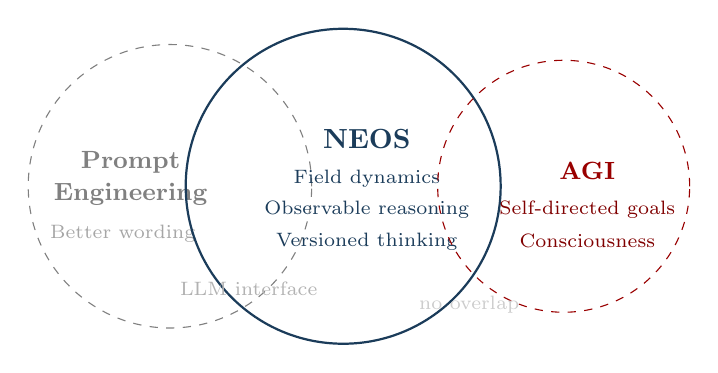
\begin{tikzpicture}
  % Prompt Engineering circle
  \draw[dashed, gray] (0,0) circle (1.8cm);
  \node[gray, font=\small\bfseries] at (-0.5,0.3) {Prompt};
  \node[gray, font=\small\bfseries] at (-0.5,-0.1) {Engineering};
  \node[gray!70, font=\scriptsize] at (-0.6,-0.6) {Better wording};

  % NEOS circle
  \draw[neosblue!60!black, thick] (2.2,0) circle (2.0cm);
  \node[neosblue!60!black, font=\bfseries] at (2.5,0.6) {NEOS};
  \node[neosblue!60!black, font=\scriptsize] at (2.5,0.1) {Field dynamics};
  \node[neosblue!60!black, font=\scriptsize] at (2.5,-0.3) {Observable reasoning};
  \node[neosblue!60!black, font=\scriptsize] at (2.5,-0.7) {Versioned thinking};

  % AGI circle
  \draw[dashed, red!60!black] (5.0,0) circle (1.6cm);
  \node[red!60!black, font=\small\bfseries] at (5.3,0.2) {AGI};
  \node[red!50!black, font=\scriptsize] at (5.3,-0.3) {Self-directed goals};
  \node[red!50!black, font=\scriptsize] at (5.3,-0.7) {Consciousness};

  % Overlap label
  \node[gray!60, font=\scriptsize] at (1.0,-1.3) {LLM interface};
  % No overlap
  \node[gray!40, font=\scriptsize] at (3.8,-1.5) {no overlap};
\end{tikzpicture}
\caption{NEOS occupies a distinct space between prompt engineering and AGI. It shares the LLM interface layer with prompt engineering but operates at a fundamentally higher level of abstraction. It does not overlap with AGI.}
\label{fig:scope}
\end{figure}

These limitations are design choices. NEOS is a specification rather than an implementation because the best implementation strategy depends on the rapidly evolving LLM ecosystem. It is not AGI because we are building a \emph{tool}, not an entity.

\subsection{Roadmap}\label{sec:roadmap}

NEOS is a beginning, not an endpoint. The roadmap spans three horizons.

\begin{figure}[H]
\centering
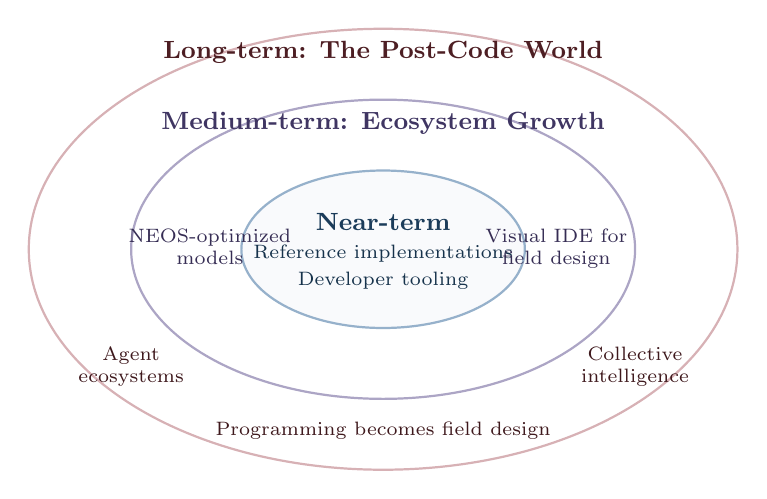
\begin{tikzpicture}
  % Outer ring
  \draw[neosred!40, thick] (0,0) ellipse (4.5cm and 2.8cm);
  \node[neosred!50!black, font=\small\bfseries] at (0,2.5) {Long-term: The Post-Code World};

  % Middle ring
  \draw[neosviolet!50, thick] (0,0) ellipse (3.2cm and 1.9cm);
  \node[neosviolet!70!black, font=\small\bfseries] at (0,1.6) {Medium-term: Ecosystem Growth};

  % Inner ring
  \draw[neosblue!50, thick, fill=neosblue!3] (0,0) ellipse (1.8cm and 1.0cm);
  \node[neosblue!60!black, font=\small\bfseries] at (0,0.35) {Near-term};
  \node[neosblue!50!black, font=\scriptsize] at (0,-0.05) {Reference implementations};
  \node[neosblue!50!black, font=\scriptsize] at (0,-0.4) {Developer tooling};

  % Medium items
  \node[neosviolet!60!black, font=\scriptsize] at (-2.2,0) {\begin{tabular}{c}NEOS-optimized\\models\end{tabular}};
  \node[neosviolet!60!black, font=\scriptsize] at (2.2,0) {\begin{tabular}{c}Visual IDE for\\field design\end{tabular}};

  % Long-term items
  \node[neosred!40!black, font=\scriptsize] at (-3.2,-1.5) {\begin{tabular}{c}Agent\\ecosystems\end{tabular}};
  \node[neosred!40!black, font=\scriptsize] at (3.2,-1.5) {\begin{tabular}{c}Collective\\intelligence\end{tabular}};
  \node[neosred!40!black, font=\scriptsize] at (0,-2.3) {Programming becomes field design};
\end{tikzpicture}
\caption{Three-horizon roadmap for NEOS development, from specification to ecosystem to paradigm.}
\label{fig:roadmap}
\end{figure}

\textbf{Near-term.} Reference implementations that run on major LLM providers. Developer tooling---IDE extensions, interactive playgrounds, tutorials. Community adoption through open specification and permissive licensing.

\textbf{Medium-term.} Models specifically fine-tuned for NEOS operation---faster dynamics computation, more faithful state maintenance, better resonance detection. A visual IDE for field design where users can drag and drop patterns, draw coupling connections, and watch dynamics in real time. A composable task marketplace where field configurations can be shared, forked, and remixed.

\textbf{Long-term.} \textbf{The post-code world.} Humans express intent in language, the NEOS shell formalizes it into field operations, LLMs execute it, and the output is meaning, not bytes. ``Programming'' becomes \emph{field design}---a creative act more like architecture than engineering. Agent ecosystems built on NEOS, where agents share reasoning states, fork each other's thinking, merge insights, and operate as a collective intelligence. The ``developer'' of the future is a field architect---someone who understands resonance dynamics, coupling stability, and collapse strategies.

\subsection{Concluding Remarks}

If the approach presented here proves viable, it may represent a transition as significant as the introduction of the operating system. The Hardware Age gave us the ability to compute. The Software Age gave us the ability to organize. The Intelligence Age will give us the ability to \textbf{reason}---systematically, observably, reproducibly.

NEOS is the first step. Not the last. The specification is open. The mathematics is grounded in decades of neural field theory~\cite{amari1977dynamics, wilson1972excitatory, coombes2005waves}. The proof-of-concept works. What remains is to build the community, iterate the specification, and push toward implementation---turning 37 markdown files into the foundation of a new computing paradigm.

\begin{calloutbox}
The last operating system will not run on silicon. It will run on \textbf{understanding}.
\end{calloutbox}

\begin{calloutbox}
If field dynamics prove to be the right abstraction for cognitive
computing, the long-term consequence is an operating system whose
primary resource is not memory or cycles, but \textbf{meaning}.
\end{calloutbox}


\section{Related Work}\label{sec:related}

NEOS draws on and extends several established research traditions. This section surveys the key areas and positions NEOS within the broader landscape.

\subsection{Neural Field Theory}

Neural field equations have been studied in computational neuroscience for over fifty years. Amari~\cite{amari1977dynamics} pioneered the study of pattern formation in lateral-inhibition type neural fields, establishing the mathematical framework of continuous activation dynamics that NEOS adopts as its computational substrate. Wilson and Cowan~\cite{wilson1972excitatory} developed foundational models of excitatory and inhibitory interactions in neural populations, providing the theoretical basis for the resonance and decay dynamics central to NEOS.

Coombes~\cite{coombes2005waves} provided a comprehensive review of waves, bumps, and patterns in neural field theories, demonstrating the rich dynamical repertoire available in continuous neural systems. Bressloff~\cite{bressloff2012spatiotemporal} extended these analyses to spatiotemporal dynamics in continuum neural fields. Sch\"{o}ner et al.~\cite{schoner2016dynamic} developed Dynamic Field Theory as a framework connecting neural dynamics to cognition and behavior, providing perhaps the closest precedent for NEOS's use of field dynamics for cognitive processing.

NEOS extends these frameworks from biological neural modeling to \emph{semantic} computing, replacing spatial coordinates with positions in meaning space and firing rates with pattern activation strengths.

\subsection{Large Language Models and Agent Frameworks}

The transformer architecture~\cite{vaswani2017attention} enabled the development of large language models with unprecedented capabilities. Brown et al.~\cite{brown2020language} demonstrated that GPT-3 could perform few-shot learning across diverse tasks, establishing LLMs as general-purpose reasoning engines. Wei et al.~\cite{wei2022chain} showed that chain-of-thought prompting elicits multi-step reasoning, revealing that LLMs can maintain and manipulate complex cognitive state.

These capabilities motivated the development of LLM-based agent frameworks. Park et al.~\cite{park2023generative} created generative agents---LLM-powered autonomous agents with memory, planning, and social interaction. Yao et al.~\cite{yao2023tree} introduced Tree of Thoughts, enabling deliberate problem solving through structured exploration of reasoning paths.

Current agent frameworks---AutoGPT, CrewAI, LangGraph, LlamaIndex---each independently reinvent state management, multi-agent coordination, and memory primitives. NEOS proposes a unifying specification that formalises the primitives these frameworks implement ad hoc.

Table~\ref{tab:agent-comparison} compares the primitives provided by
prominent agent frameworks.  AutoGPT~\cite{autogpt2023} introduced
autonomous goal decomposition and persistent memory.
CrewAI~\cite{crewai2024} added role-based multi-agent coordination.
LangGraph~\cite{langgraph2024} provides stateful, graph-structured
agent workflows.  LlamaIndex~\cite{llamaindex2023} specialises in
retrieval-augmented generation with structured data connectors.  Each
framework addresses a subset of the operating-system primitives
(memory, scheduling, multi-agent coordination) that NEOS aims to
unify; none provides observable dynamics, attractor detection, or
formal stability conditions such as
Equation~\eqref{eq:coupling-stability-multi}.

\begin{table}[htbp]
\centering
\caption{Primitive comparison across agent frameworks.  \checkmark\
  = natively supported; $\circ$ = partial or plugin-based; --- = absent.}
\label{tab:agent-comparison}
\small
\begin{tabular}{@{}lccccc@{}}
\toprule
\thead{Primitive} & \thead{AutoGPT} & \thead{CrewAI} & \thead{LangGraph}
  & \thead{LlamaIndex} & \thead{NEOS} \\
\midrule
Persistent memory       & \checkmark & $\circ$ & \checkmark & \checkmark & \checkmark \\
Multi-agent coordination & ---       & \checkmark & \checkmark & $\circ$ & \checkmark \\
Tool use                & \checkmark & \checkmark & \checkmark & \checkmark & \checkmark \\
Observable dynamics     & ---        & ---     & ---        & ---        & \checkmark \\
Attractor detection     & ---        & ---     & ---        & ---        & \checkmark \\
Formal stability        & ---        & ---     & ---        & ---        & \checkmark \\
\bottomrule
\end{tabular}
\end{table}

\subsection{Context and Prompt Engineering}

Reynolds and McDonell~\cite{reynolds2021prompt} characterized prompt programming as a new paradigm for interacting with language models, exploring strategies beyond few-shot prompting. While this work recognized the importance of structured interaction with LLMs, it remained within the paradigm of text-based prompting.

More recently, Kimai~\cite{kimai2025context} framed \emph{context engineering} as the broader discipline that subsumes prompt engineering, defining context as the complete information payload provided to an LLM at inference time.  That work organises the progression from single prompts (atoms) through persistent memory (cells) and multi-step orchestration (organs) to neural fields and protocol shells---a hierarchy that closely mirrors the evolution hierarchy presented in Section~\ref{sec:evolution}.  NEOS builds on this vision by providing the formal substrate---field dynamics, attractor detection, and collapse operators---that turns the context-engineering progression from a pedagogical metaphor into an executable specification.

NEOS argues that prompts are the assembly language of the Intelligence Age. Field dynamics, with their mathematical precision, observable state, and composable operations, constitute the high-level language. The transition from prompt engineering to field dynamics parallels the historical transition from assembly language to structured programming~\cite{silberschatz2018operating}.

\subsection{Operating System Abstraction History}

The classical operating systems literature~\cite{silberschatz2018operating} documents a consistent trajectory: each generation of OS abstracts away the bottleneck of its era. Early operating systems managed hardware resources (CPU scheduling, memory allocation). Later systems managed software complexity (processes, threads, virtual memory, file systems). NEOS continues this trajectory into the Intelligence Age, where the bottleneck is \emph{meaning}---and the OS must manage semantic fields, resonance relationships, and cognitive state.

The analogy between NEOS and the Java Virtual Machine (Section~\ref{sec:analogy}) extends the OS abstraction principle: just as the JVM decoupled code from hardware, NEOS decouples reasoning from any specific LLM.

\subsection{Quantum Cognition}

Busemeyer and Bruza~\cite{busemeyer2012quantum} developed quantum models of cognition and decision, demonstrating that quantum probability theory can capture phenomena---such as order effects, interference, and entanglement---that classical probability cannot. Pothos and Busemeyer~\cite{pothos2013can} argued that quantum probability provides a genuinely new direction for cognitive modeling, not merely a mathematical convenience.

NEOS's quantum semantics pillar draws directly from this tradition. Superposition (multiple interpretations coexisting before collapse), non-commutativity (injection order affecting outcomes), and observer-dependent collapse (strategy choice shaping results) are not loose metaphors in NEOS---they are operational design principles inspired by quantum probability theory, implemented via the field equation rather than via Hilbert-space operators with precise mathematical definitions in terms of the field equation. The connection between neural field dynamics and quantum-inspired cognition that NEOS establishes appears to be novel.

\subsection{Cognitive Architectures}

Classical cognitive architectures provide structured frameworks for
modeling human cognition.  ACT-R~\cite{anderson2007how} decomposes
cognition into declarative memory, procedural rules, and a
production-matching cycle that governs behavior.
Soar~\cite{laird2012soar} models cognition as a problem-space search
augmented by chunking (automatic rule formation) and episodic memory.
CLARION~\cite{sun2006clarion} uniquely combines explicit rule-based
and implicit connectionist subsystems, capturing the dual-process
nature of human cognition.

These architectures share with NEOS the commitment to making cognitive
processing structured and inspectable.  However, they were designed for
rule-based or symbolic substrates, not for LLMs.  NEOS can be viewed as
extending the cognitive-architecture tradition to LLM-based systems:
replacing production rules with field dynamics, working memory with
activation landscapes, and goal stacks with attractor basins.

\subsection{Attractor Dynamics}

Hopfield~\cite{hopfield1982neural} demonstrated that neural networks with symmetric connections exhibit attractor dynamics, where the network converges to stable states that function as associative memories. Khona and Fiete~\cite{khona2022attractor} reviewed the role of attractor and integrator networks in the brain, connecting theoretical models to empirical neuroscience.

NEOS's attractor detection mechanism extends this tradition from fixed-point dynamics in discrete networks to emergent structure in continuous semantic fields. The seven attractor basins discovered in the software quality session (Section~\ref{sec:evidence}) demonstrate that Hopfield-style attractor dynamics generalize naturally to the domain of meaning and reasoning.


\section*{Acknowledgements}

The author gratefully acknowledges David Kimai's
\emph{Context-Engineering} handbook~\cite{kimai2025context}, whose
first-principles exploration of context design, orchestration, and the
biological progression from atoms to neural fields provided key
inspiration for the NEOS framework.

\appendix
% ══════════════════════════════════════════════════════════════════
%  Appendix A — Detailed Session Walkthroughs
% ══════════════════════════════════════════════════════════════════

\section{Detailed Session Walkthroughs}\label{app:sessions}

This appendix presents wave-by-wave transcripts for both case studies.
All terminal output is reproduced from actual session logs; no numbers
have been edited.

% ══════════════════════════════════════════════════════════════════
%  A.1 — Software Quality Discipline
% ══════════════════════════════════════════════════════════════════

\subsection{Software Quality --- Wave-by-Wave}\label{app:sw-waves}

\subsubsection*{Setup: Creating the Field}

\begin{terminalbox}[Field Creation and Parameter Tuning]
\begin{lstlisting}[style=neosshell]
nf session new "software_quality_discipline"
[SESSION] Created: software_quality_discipline

nf field create quality_field
[FIELD] Created: $quality_field
  Parameters: l=0.05  a=0.30  t=0.40  s=0.50  (defaults)

nf tune lambda=0.04 alpha=0.35 tau=0.35 sigma=0.40
[TUNE] l=0.04  a=0.35  t=0.35  s=0.40
\end{lstlisting}
\end{terminalbox}

\noindent
The tuning creates a \emph{retentive} ($\lambda = 0.04$, slower decay),
\emph{strongly resonant} ($\alpha = 0.35$), \emph{inclusive}
($\tau = 0.35$, lower threshold), and \emph{selective}
($\sigma = 0.40$, tighter bandwidth) field---ideal for discovering which
software engineering patterns genuinely cohere.

\subsubsection*{Wave~1: Defensive Quality (p001--p006, Cycles 1--3)}

Six code-review patterns are injected.  The full 15-pair resonance
matrix is computed at injection time:

\begin{terminalbox}[Wave 1 --- Resonance Matrix]
\begin{lstlisting}[style=neosshell]
nf inject "correctness" 0.90
[INJECT] correctness (s: 0.90) -- p001

nf inject "edge_case_handling" 0.85
[INJECT] edge_case_handling (s: 0.85) -- p002
  [RESONANCE] <-> @correctness: R = 0.82 STRONG

nf inject "security_no_injection_vectors" 0.95
[INJECT] security_no_injection_vectors (s: 0.95) -- p003
  [RESONANCE] <-> @correctness:        R = 0.68 MODERATE
  [RESONANCE] <-> @edge_case_handling:  R = 0.74 STRONG

nf inject "input_validation" 0.90
[INJECT] input_validation (s: 0.90) -- p004
  [RESONANCE] <-> @security_no_injection: R = 0.91 STRONG

RESONANCE MATRIX (15 unique pairs):
  Peak: @security <-> @input_validation = 0.91
  STRONG: 8/15 (53%)  MODERATE: 7/15 (47%)
  WEAK: 0  INHIBIT: 0
\end{lstlisting}
\end{terminalbox}

\begin{terminalbox}[Wave 1 --- Dynamics (3 Cycles)]
\begin{lstlisting}[style=neosshell]
nf cycle 3 --trace
[CYCLE 1] C = 0.42  (LOW->MEDIUM)
  All 6 amplified -- no isolation.
[CYCLE 2] C = 0.58  (MEDIUM, cross-cluster links forming)
[CYCLE 3] C = 0.71  (HIGH)

  [ATTRACTOR-EMERGED] "defensive_quality"
    Core: {@security_no_injection, @input_validation,
           @edge_case_handling, @correctness,
           @no_leaked_secrets, @error_handling}
    Coherence: 0.71
\end{lstlisting}
\end{terminalbox}

\subsubsection*{Wave~2: Building Breadth (p007--p014, Cycles 4--8)}

Eight patterns expand the field.  A 4-tier energy stratification
emerges, with the \emph{performance dyad}
(\texttt{@no\_n\_plus\_1}, \texttt{@no\_alloc}) permanently
stationed as an asymptotic satellite:

\begin{terminalbox}[Wave 2 --- Dynamics (5 Cycles)]
\begin{lstlisting}[style=neosshell]
nf cycle 5 --trace
[CYCLE 4] C = 0.52  (8 new patterns integrating)
[CYCLE 5] C = 0.60  (threshold crossing)
[CYCLE 6] C = 0.67  (sub-attractor forming in core 12)
[CYCLE 7] C = 0.74
  [ATTRACTOR-EMERGED] "holistic_quality_discipline"
    Core: 12 patterns (SECURITY + LOGIC + CLARITY + KEYSTONE)

[CYCLE 8] C = 0.79  (STABLE)
  4-tier energy stratification:
    Tier 1: security+logic core (ceiling)
    Tier 2: clarity+design (converging)
    Tier 3: @test_coverage (keystone bridge)
    Tier 4: performance dyad (satellite, ~0.69-0.76)
\end{lstlisting}
\end{terminalbox}

\subsubsection*{Wave~3: Refactoring (p015--p022, Cycles 9--11)}

The field's strongest bond emerges at injection:
\texttt{@behavior\_preservation} $\leftrightarrow$
\texttt{@tests\_before\_refactoring} at $R = 0.94$.

\begin{terminalbox}[Wave 3 --- Field Maximum Bond]
\begin{lstlisting}[style=neosshell]
nf inject "behavior_preservation" 0.92
[INJECT] behavior_preservation (s: 0.92) -- p015
  [RESONANCE] <-> @tests_before_refactoring: R = 0.94  FIELD MAX

nf cycle 3 --trace
[CYCLE  9] C = 0.62  (22 patterns integrating)
[CYCLE 10] C = 0.71  (attractor forming across 20 patterns)
[CYCLE 11] C = 0.80
  [ATTRACTOR-EVOLVED] "holistic_quality_discipline" -> MATURE
    Core: 20/22 patterns.  Saturated: 11 at ceiling.
\end{lstlisting}
\end{terminalbox}

\subsubsection*{Wave~4: Testing Mirror (p023--p031, Cycles 12--18)}

Nine testing patterns trigger echo detection---the functor~$F$
begins mapping production $\to$ testing:

\begin{terminalbox}[Wave 4 --- Mass Saturation at Cycle 14]
\begin{lstlisting}[style=neosshell]
nf inject "test_behavior_not_implementation" 0.90
[INJECT] test_behavior_not_implementation (s: 0.90) -- p028
  ECHO: mirrors @behavior_preservation (production)

nf cycle 7 --trace
[CYCLE 14] C = 0.79
  MASS SATURATION: 7 patterns reach ceiling simultaneously
[CYCLE 15] C = 0.85
  [ATTRACTOR-EVOLVED] -> DOMINANT (29/31 core, 25 at ceiling)
[CYCLE 18] C = 0.91  -- 6-layer topology confirmed
\end{lstlisting}
\end{terminalbox}

\subsubsection*{Wave~5: OOP/SOLID and First Absorptions (p032--p040, Cycles 19--30)}

The OOP wave produces three absorptions.  S, I, and D are
\emph{rediscovered}---they already exist in the field before SOLID
is named:

\begin{terminalbox}[Wave 5 --- Three Absorptions]
\begin{lstlisting}[style=neosshell]
nf inject "single_responsibility_principle" 0.88
[ABSORBED] -> @single_responsibility (p008)
  R=0.98 -- exact duplicate.  ABSORPTION #1

nf inject "interface_segregation_principle" 0.82
[ABSORBED] -> @api_minimal (p010)
  R=0.96.  ISP and minimal API are the SAME THING.
  ABSORPTION #2

nf inject "law_of_demeter_minimal_knowledge" 0.78
[ABSORBED] -- distributed across THREE patterns:
  @encapsulation /\ @api_minimal /\ @dependency_direction
  Combined coverage: 94%.  TYPE: DECOMPOSITION.
  ABSORPTION #3

nf cycle 6 --trace   # cycles 25-30
[CYCLE 30] C = 0.955 (pre-Singleton)
  Field constant: R_pt = 0.88  |  Selection function: r = 0.94
\end{lstlisting}
\end{terminalbox}

\subsubsection*{Waves~6--7: Great Convergence and Final Absorptions
  (p046--p062, Cycles 34--52)}

Ten GoF patterns (Wave~6) produce the ``Great Convergence''---14
patterns reaching ceiling in 10~cycles.  The Golden Pair (Strategy +
Decorator) converge simultaneously with 5/5 SOLID locks each:

\begin{terminalbox}[Waves 6--7 --- Great Convergence]
\begin{lstlisting}[style=neosshell]
nf inject "strategy_interchangeable_algorithms" 0.88
[INJECT] strategy (s: 0.88)
  9 STRONG bonds -- new resonance record
  Resonates with ALL FIVE SOLID principles

nf cycle 10 --trace   # cycles 34-43
[CYCLES 37-39] "The Golden Pair"
  @strategy + @decorator -> ceiling SIMULTANEOUSLY
  Both 5/5 SOLID locks -- only patterns with perfect alignment
  C = 0.984  |  52 at ceiling

# Wave 7: four self-referential absorptions
nf inject "coupling_to_abstraction_not_concretion" 0.86
[ABSORBED] -> @dependency_inversion (p008)
  DIP APPLIED TO ITSELF:
    The field held the ABSTRACTION (@dependency_inversion).
    The injection offered a CONCRETION (a specific rephrasing).
    The field coupled to its abstraction and rejected the
    concretion.
  Self-referential events: 4/7 (57%)
\end{lstlisting}
\end{terminalbox}

% ══════════════════════════════════════════════════════════════════
%  A.2 — PCAP Analysis
% ══════════════════════════════════════════════════════════════════

\subsection{PCAP Analysis --- Wave-by-Wave}\label{app:pcap-waves}

\subsubsection*{Wave~1: Network Core (p001--p003, Cycles 1--3)}

Three foundational patterns seed the field: raw capture, protocol
decode, and DNS resolution.  The field runs on \textbf{default
parameters}---no tuning.

\begin{terminalbox}[PCAP Wave 1 --- First Attractor]
\begin{lstlisting}[style=neosshell]
nf inject "packet_capture" 0.9
[INJECT] packet_capture (s: 0.90) -- p001

nf inject "protocol_mapping" 0.9
[INJECT] protocol_mapping (s: 0.90) -- p002
  [RESONANCE] <-> @packet_capture: R = 0.72 STRONG

nf inject "dns_resolution" 0.9
[INJECT] dns_resolution (s: 0.90) -- p003

[RESONANCE MATRIX]
                     capture   mapping   dns
  @packet_capture   [ 1.00      0.72     0.68 ]
  @protocol_mapping [ 0.72      1.00     0.81 ]
  @dns_resolution   [ 0.68      0.81     1.00 ]

  Strongest: @protocol_mapping <-> @dns_resolution (R=0.81)

nf cycle 3 --trace
[CYCLE 1] C = 0.52  (MEDIUM)
  @protocol_mapping: 0.855 -> 0.904 (+0.049)
[CYCLE 2] C = 0.61  (MEDIUM-HIGH)
  Hub forming: @protocol_mapping at 0.919 (dominant)
[CYCLE 3] C = 0.71  (HIGH)

  [ATTRACTOR-EMERGED] "network_analysis_core"
    Core: {@protocol_mapping, @dns_resolution,
           @packet_capture}
    Coherence: 0.71
    Hub: @protocol_mapping (0.936)
\end{lstlisting}
\end{terminalbox}

\subsubsection*{Wave~2: IP Enrichment and Rescue (p004--p006, Cycles 4--6)}

\texttt{@ip\_geolocalization} is injected at 0.50---the weakest pattern
in the field.  Its $R = 0.94$ bond with \texttt{@ip\_lookup} rescues it
from near-expulsion:

\begin{terminalbox}[PCAP Wave 2 --- Rescue and Hub Migration]
\begin{lstlisting}[style=neosshell]
nf inject "ip_geolocalization" 0.5
[INJECT] ip_geolocalization (s: 0.50) -- p006
  WARNING: Low activation (threshold t=0.40)

  [RESONANCE: @ip_geolocalization]
    <-> @ip_lookup:  R=0.94 [VERY STRONG]  <- lifeline
    <-> @abuse_ip:   R=0.79 [STRONG]
    <-> @dns_resolution: R=0.61 [MODERATE]

nf cycle 3 --trace
[CYCLE 4]
  @ip_geolocalization: 0.475 -> 0.587 (+0.112) -- rescue
  @ip_lookup: 0.855 -> 0.948 (+0.093)

[CYCLE 5]
  HUB MIGRATION: @protocol_mapping -> @ip_lookup
  @ip_lookup now highest activation (0.987)
  @ip_geolocalization: 0.558 -> 0.691 (+0.133)

[CYCLE 6] C = 0.82
  [ATTRACTOR-MERGED] "pcap_analysis_engine"
    Absorbed: "network_analysis_core" + "ip_enrichment"
    Hub: @ip_lookup (0.998)
    Coherence: 0.82
\end{lstlisting}
\end{terminalbox}

\subsubsection*{Wave~3: Security and Inspection (p007--p009, Cycles 7--9)}

Security patterns produce a dual-hub structure and the field's first
eigenspectrum:

\begin{terminalbox}[PCAP Wave 3 --- Eigenstructure Emerges]
\begin{lstlisting}[style=neosshell]
nf inject "suspicious_dns" 0.8
[INJECT] suspicious_dns (s: 0.80) -- p007
  <-> @dns_resolution: R=0.93 [VERY STRONG]
  <-> @abuse_ip:       R=0.87 [VERY STRONG]

nf inject "payload_analysis" 0.7
[INJECT] payload_analysis (s: 0.70) -- p009
  <-> @packet_capture:     R=0.95 [VERY STRONG]  <- field max
  <-> @protocol_mapping:   R=0.89 [VERY STRONG]

nf cycle 3 --trace
[CYCLE 8] C = 0.84
  Dual-hub: @protocol_mapping (0.998), @ip_lookup (0.998)

[CYCLE 9] C = 0.89
  Eigenspectrum:
    l1 = 6.12 (dominant unified mode)
    l2 = 0.89 (security subspace)
    l3 = 0.54 (enrichment subspace)

  [ATTRACTOR-CONSOLIDATED] "pcap_security_analyzer"
    Dual-hub: @protocol_mapping (0.998), @ip_lookup (0.998)
    4 functional layers integrated
\end{lstlisting}
\end{terminalbox}

\noindent
The four layers---Acquisition, Processing, Enrichment,
Security---emerged from resonance dynamics alone, not from any
injected topology.

\subsubsection*{Wave~4: Threat Classification and Triple-Hub
  (p010, Cycles 10--12)}

The final pattern completes the threat-hunting pipeline:

\begin{terminalbox}[PCAP Wave 4 --- Triple-Hub Formation]
\begin{lstlisting}[style=neosshell]
nf inject "malware_analysis" 0.8
[INJECT] malware_analysis (s: 0.80) -- p010
  <-> @payload_analysis: R=0.91 [VERY STRONG]
  <-> @abuse_ip:         R=0.88 [VERY STRONG]
  <-> @suspicious_dns:   R=0.86 [VERY STRONG]

nf cycle 3 --trace
[CYCLE 10] C = 0.88
  @malware_analysis: 0.760 -> 0.882 (+0.122) -- rapid
  @abuse_ip rising to 0.998 -- threat hub forming

[CYCLE 11] C = 0.91
  Triple-hub structure confirmed:
    @protocol_mapping  0.998 -- structural/parsing hub
    @ip_lookup         0.998 -- enrichment/metadata hub
    @abuse_ip          0.998 -- threat intelligence hub

[CYCLE 12] C = 0.93 [EXCELLENT]
  Eigenspectrum:
    l1 = 7.84 (dominant unified mode)
    l2 = 0.92 (threat subspace)
    l3 = 0.71 (enrichment subspace)
    l4 = 0.53 (inspection subspace)
    Gap ratio: l1/l2 = 8.52 (highly stable)

  [ATTRACTOR-REINFORCED] "pcap_security_analyzer"
    Triple-hub unified field (10 patterns)

    @abuse_ip          0.998  -- threat intelligence hub
    @protocol_mapping  0.998  -- structural parsing hub
    @ip_lookup         0.998  -- enrichment hub
    @dns_resolution    0.997  -- protocol core
    @packet_capture    0.995  -- data acquisition
    @suspicious_dns    0.992  -- anomaly detection
    @payload_analysis  0.989  -- deep packet inspection
    @unsecure_protocols 0.978 -- vulnerability assessment
    @ip_geolocalization 0.963 -- geographic context
    @malware_analysis  0.962  -- threat classification

    Coherence: 0.93  |  Stability: EXCELLENT
\end{lstlisting}
\end{terminalbox}

\noindent
Three independent analysis perspectives---structural parsing,
enrichment, and threat intelligence---converge to 0.998.  The
eigenvalue gap ratio $\lambda_1/\lambda_2 = 8.52$ confirms this is a
deeply stable configuration.  From this collapsed attractor, NEOS
identified an active AsyncRAT~v6.1.0~Pro infection with confirmed
C2~infrastructure at \texttt{206.123.152.51:3980}.


\bibliographystyle{plainnat}
\bibliography{bibliography}

\end{document}
